\documentclass{lalabook}
\usepackage[utf8]{inputenc}


\usepackage{geometry}
\geometry{a5paper, inner=15mm, outer=11mm, top=17mm, bottom=17mm}

\setlength{\parindent}{0em}
\setlength{\parskip}{1ex}


\usepackage[hidelinks]{hyperref}

\usepackage{epigraph}
\setlength\epigraphwidth{.95\textwidth}
\setlength\epigraphrule{0pt}
\renewcommand{\textflush}{flushright}

\usepackage{graphicx}
\graphicspath{ {../images/} }
\usepackage{wrapfig}
\usepackage[font=scriptsize]{caption}
\usepackage{subcaption}

\usepackage{xcolor}
\usepackage{normalcolor}

\newenvironment{sectcredits}
{\vspace{1cm} \vfill \footnotesize \begin{description}}
{\end{description}}

\usepackage{enumitem}

\usepackage{tikz}

 \usepackage{fontspec}
 \setmainfont{Quicksand}[
 ItalicFont = Montserrat Light Italic
 ]
 % Fonts that need to be installed in the system:
 % Quicksand     https://fonts.google.com/specimen/Quicksand
 % Montserrat     https://fonts.google.com/specimen/Montserrat
 

\usepackage{fancyhdr}

\pagestyle{fancy}
\fancyhf{}
\fancyhead[LE,RO]{\bfseries \small \rightmark}
\fancyfoot[LE,RO]{\bfseries \large \thepage}
\renewcommand{\headrulewidth}{0pt}


\usepackage{tocloft}
\renewcommand{\cftdot}{}

\renewcommand\cfttoctitlefont{\bfseries \Large}
\renewcommand\cftsecfont{\large}
\renewcommand\cftsecpagefont{\large}

\setlength\cftparskip{3pt}
\setlength\cftbeforetoctitleskip{-3em}
\setlength\cftaftertoctitleskip{1em}
\setlength\cftsecindent{0pt}
\renewcommand\cftsecafterpnum{\hspace*{8em}}

%If using babel: put the next command inside the braces of
%\addto\captionsenglish{  }
%substituting "english" by the language set in babel
\renewcommand*\contentsname{Exhibits page index:} 

\setcounter{tocdepth}{1} % Show only sections

\begin{document}

\thispagestyle{empty}
\noindent
\begin{tikzpicture}[remember picture, overlay]
 	\node[inner sep=0pt] at (current page.center) {
\includegraphics[width=\paperwidth,height=\paperheight]{cover_blank}};
	\node at (current page.north east) [anchor=north east, xshift=-6mm, yshift=-8mm, font=\Large\bfseries]{\color[rgb]{1,1,1}EXHIBITION BOOKLET};
	\node at (current page.north east)  [anchor=north east, xshift=-6mm, yshift=-132mm, align=left, font=\Huge\bfseries]  {THE MATHEMATICS \\ OF MUSIC};
	%\node at (4.2,-11.6) [anchor=west] {\Huge \bf OF MUSIC};
\end{tikzpicture}


\newpage

\epigraph{ \itshape ``Mathematics and music, the most sharply contrasted fields of scientific activity which can be found, and yet related, supporting each other, as if to show forth the secret connection which ties together all the activities of our mind, and which leads us to surmise that the  manifestations of the artist's genius are but the unconscious expressions of a mysteriously acting rationality.''
}
{\vspace{0.5em}Hermann von Helmholtz (1821 - 1894) \\
a \textit{Vorträge und Reden} (1884, 1896), Vol 1, p 122.}

La música i les matemàtiques comparteixen molts atributs com a camps d'estudi. Les dues disciplines estudien objectes abstractes, tenen estructures complexes i les seves pròpies normes per a la seva manipulació, una notació clarament definida, i són absolutament precises als seus resultats. Treballar a les dues requereix pràctica, creativitat i una ment analítica. Vist això, no és cap sorpresa que la música i les matemàtiques estan estretament relacionades.

La seva relació va molt més enllà de les habilitats necessàries per al seu estudi. Les matemàtiques estan profundament lligades a la música, des de les físiques del so fins a la construcció d'instruments, des de patrons rítmics fins a l'harmonia tonal, des de la música clàssica fins a l'electrònica. Les matemàtiques formen la base de la música i el nostre enteniment de l'art de la mateixa manera que sosté la física i el nostre enteniment del món.

Escoltar música amb oïda matemàtica porta a l'amant de la música a una comprensió més profunda, amb apreciació dels detalls, a un major gaudi de l'art; i als professionals l'habilitat de compondre i eines per  expressar la seva creativitat.

\begin{flushright}
IMAGINARY, 2019 %update 2021 ?
\end{flushright}

\vfill
La La Lab - Les Matemàtiques de la Música / Booklet d'exhibició \\
IMAGINARY, \url{www.imaginary.org}, \href{mailto:info@imaginary.org}{info@imaginary.org} \\
Versió 0.5CAT, \today / Llicència: CC BY-SA


\section*{La La Lab - Les Matemàtiques de la Música}

Pensat en col·laboració amb experts en investigació de la música i les matemàtiques, La La Lab combina el format de laboratori amb exposicions interactives. Per aquest motiu podem revelar les impressionants connexions entre les matemàtiques i la música tot impulsant la creativitat musical i el coneixement matemàtic.

La la Lab és una experiència de laboratori modular. Aquest booklet t'ajudarà a donar una ullada més profunda. Hi pots trobar informació complementària sobre cada mòdul, enllaços per descobrir característiques addicionals i lectures recomanades. Si us plau, agafa'n una còpia o descarrega'l del nostre web. l'exposició és open source i està disponible sota llicències gratuïtes. Pots trobar tot el software, imatges, text i dades 3D a: \url{lalalab.imaginary.org}

IMAGINARY és una organització sense ànim de lucre per a la comunicació interactiva, oberta, artística i col·laborativa de les matemàtiques modernes dirigides al públic general. Creat el 2007 al Mathematische Forschungsinstitut Oberwolfach, un institut a Libniz, IMAGINARY ha rebut múltiples guardons per la seva contribució a la divulgació científica. Des del 2008 s'han organitzat més de 340 activitats en més de 60 països i en 30 idiomes, arribant a milions de visitants.


\section*{La La Lab Crèdits}
\footnotesize
Una exposició creada per IMAGINARY.
Presentat per la fundació Heidelberg Laureate Forum Foundation.
El desenvolupament de l'exposició i la producció dels mitjans s'ha fet possible gràcies al suport de la fundació Klaus Tschira Stiftung.

\paragraph{Comitè d'experts i mòduls:}
Moreno Andreatta (CNRS / IRCAM / Sorbonne University and USIAS / IRMA / University of Strasbourg), Manuela Donoso (Brooklyn Research), Thomas Noll (ESMUC Barcelona, TU Berlin), Luisa Pereira (New York University), Jürgen Richter-Gebert (TU München).


\paragraph{Equip IMAGINARY:}
Andreas Matt (Director), Daniel Ramos (Curador, Recerca), Kathrin Unterleitner (Gestió de projectes), Bianca Violet (Contingut, Comunicació), Christian Stussak (Software, Exposicions), Eric Londaits (Software, Exposicions), Sebastián Uribe (Consell tècnic, Exposicions), Malte Westphalen (Escenografia, Disseny), Konrad Renner (Disseny), Tobias Hermann (Hardware), Lukas Reck (Producció, LLum i So), Daniel Weiss (Producció), Antonia Mey (Assistència), Magdalena Hreczynska (Assistència).

\paragraph{Mòduls:}
Corentin Guichaoua (Univ. Strasbourg), Philipp Legner (Mathigon), Patrick Wilson, Aaron Montag and Konrad Heidler (TU
 München), Gerhard Widmer, Stefan Balke, Carlos Eduardo Cancino Chacón and Florian Henkel (JKU Linz), Neil Sloane (OEIS Foundation), Neil Thapen (Academy of Sciences of the Czech Republic), Vitor Guerra Rolla, Pedro Arthur and José Ezequiel Soto Sánchez (Visgraf Lab, Instituto de Matemática Pura e Aplicada, Rio de Janeiro), Ryan Cashman (Nano Animal).

\paragraph{Textos del booklet:}
Daniel Ramos, Sebastián Uribe, Kathrin Unterleitner, Andreas Daniel Matt, Bianca Violet and Eric Londaits (IMAGINARY), Jürgen Richter-Gebert (TU Munich), Pedro Arthur, Vitor Guerra Rolla, and José Ezequiel Soto Sánchez (Visgraf Lab, IMPA), Gerhard Widmer (JKU Linz), Thomas Noll (ESMUC Bar\-ce\-lo\-na, TU Berlin), Ryan Cashman (Nano Animal), Manuela Donoso (Brookly Research), Luisa Pereira (New York University).

\paragraph{Traducció al català:} David Fornell.

\paragraph{Agraïments:}
Heidelberg Laureate Forum Foundation.

\paragraph{Amb el suport de:}
Technische Universität München, Springer Publishing House, The Looking Glass, Taylor \& Francis Publishing House.

\paragraph{Agraïments:}
Alba Málaga Sabogal, Yann Orlarey, Catinca Dumitrascu, Google Magenta Team, Tero Parviainen, Ricardo Dodds, Exploratorium San Francisco, all film authors, European Research Council (ERC), project no.670035.

Els continguts de l'exposició estan disponibles sota llicències open source.
\normalsize


\section{The Spectrum of Sound}

Sound is a vibration of some body transmitted through the air and perceived by your ears. If you move up and down your hand once per second, we say that your hand vibrates at a frequency of 1 Hertz (Hz). If you move it up and down twice per second, the frequency is 2 Hz. If you could do it about 20 times per second (20 Hz), your eardrums would start sensing the vibration transmitted through the air. Probably you can do it with your hand, but you can use a string on a guitar, the membrane of a drum, the air inside a flute, your vocal folds, the body of a bell... Typically a human can hear vibrations with a frequency between 20 and 20 000 Hz. The higher the frequency, the higher the pitch of the sound.

However, if you use a guitar string or a flute as vibrating bodies, the sound you will perceive will be very different in each of the two cases. This is because we almost never hear a ``pure'' frequency, any natural sound is a mixture of vibrations at different frequencies and varying intensities. A guitar string tuned at a middle A note, will vibrate at 440 Hz. This is the fundamental frequency, but the string will inevitably vibrate also at 880 Hz (the double), 1320 Hz (the triple), and with all the multiple frequencies (called harmonic frequencies), but with less intensity each time. A flute will also vibrate at all these frequencies, but with different intensities. It is the varying intensities of the harmonic frequencies that makes our ear distinguish between guitar and flute. The set of frequencies with their intensities is called the spectrum of the sound, and it defines what we call timbre in music.

What would be a ``pure'' sound, just one frequency and no ``contamination'' from others? Mathematically, we can describe this sound as a sinusoidal wave. It is the sound that would make a perfectly elastic spring that could vibrate without losing any energy. We can't build such a spring, but we can make the membrane of a speaker vibrate at this pure frequency using electronics. A surprising, yet totally useful result in mathematics, is that every periodic function of period $2\pi$ can be approximated by summing up a sequence of sine waves if they are scaled and shifted appropriately. In a formula: 
$$g(t) \approx A_0 + \sum_{i=1}^N A_i \cdot \sin(i t + \varphi_i).$$


This implies that by adding appropriate sine waves we can simulate any static sound, the only information needed is the set of intensities $A_i$ and the phase shifts $\varphi_i$. This has deep implications. On the one hand it allows us to decompose of a complex signal into many simpler ones in a very structured way. Thus, it makes things much simpler to analyze and understand. On a more abstract level it connects different spaces: the time space where signals are described by values (like air pressure) changing over time and the frequency space where signals are composed from simpler ones. Depending on the situation it might be way easier to address a certain problem in one space or the other.

Its applications are far reaching and cover many diverse areas besides sound and music, such as communication technology, quantum theory, coding theory, statistics, electrical circuit design, and an endless series of other topics.

\begin{wrapfigure}{l}{0.35\textwidth}
\centering
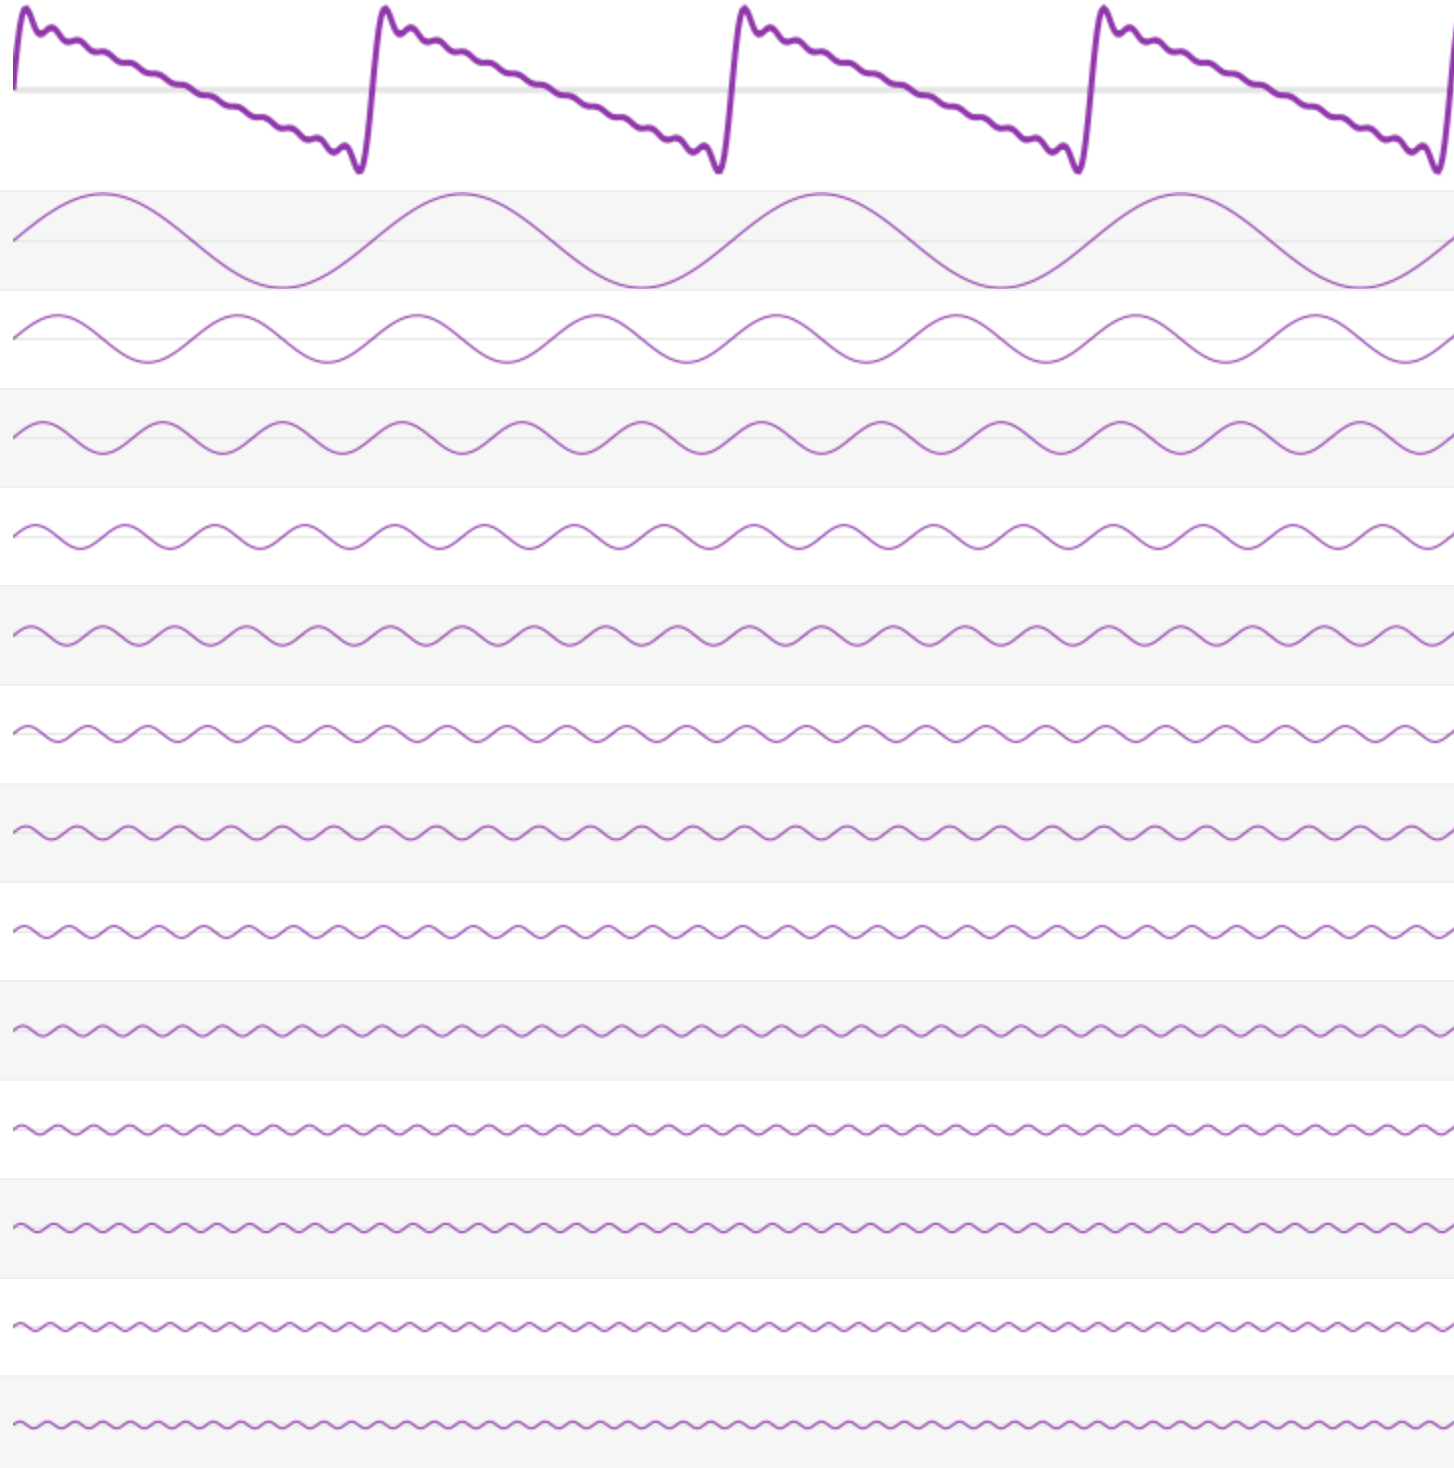
\includegraphics[width=0.35\textwidth]{SpectrumOfSound_1}
\caption*{A sawtooth wave as a sum of sine waves.}
\end{wrapfigure}
On the first screen of the exhibit, you can try to generate a wave by adding harmonic frequencies. Use just one frequency (sine) to hear a ``mathematically pure'' sound. Adjust the intensity of each of the harmonic frequencies, or click on the square or sawtooth waves, to hear different timbres. 

Heuristically, a string instrument has more intense harmonics, and wind instruments have less intense harmonics. But anyway, we are still far from a full synthesizer. To simulate a real instrument, we have to take into account that the sound is not static and eternal, it starts at some point, increases in intensity, then it decays and fades out. So, frequencies and their intensities change through time. Instruments such as bells, xylophones and most percussions do not have a spectrum formed by multiples of a fundamental frequency, but other frequencies depending on the geometric shape of the vibrating body. Therefore, it is quite difficult to synthesize a real instrument.

However, there is an extraordinary mathematical tool that allows us to reverse the process. Instead of adding up frequencies to obtain a composed signal, the Fourier transform is a procedure that allows to take an arbitrary signal (recorded with a microphone, for instance) and to decompose it into its fundamental pieces: the frequencies and their intensities that you would need to use to generate the signal using pure frequencies as building blocks. 

Let $g(t)$ be a signal represented as a function, so that for each time t it returns the intensity of the sound (this intensity may be the air pressure, or the voltage in the line wire of a microphone). The Fourier transform of a signal $g(t)$ is a new function $\hat g(t)$ that for each frequency $f$ returns the intensity of a sine wave with that frequency required to synthesize the signal $g(t)$. It is achieved with this formula:
$$\hat g(f) = \int_{-\infty}^{\infty} g(t)\ e^{2\pi i f t } \ dt$$

Note that there are complex values inside the integral, so that the Fourier transform is a complex-valued function. This is because there are two pieces of information needed to synthesize a signal: the amplitude $A_i$ and the phase shifts $\varphi_i$. 

The Fourier transform gives both the amplitude and phase of the signal as modulus and argument of the complex value. Usually, for audio analysis often only the modulus is used to obtain a graph with peaks at the most prominent frequencies, which is sufficient to reconstruct the original signal with accuracy.

\begin{wrapfigure}{r}{0.45\textwidth}
\centering
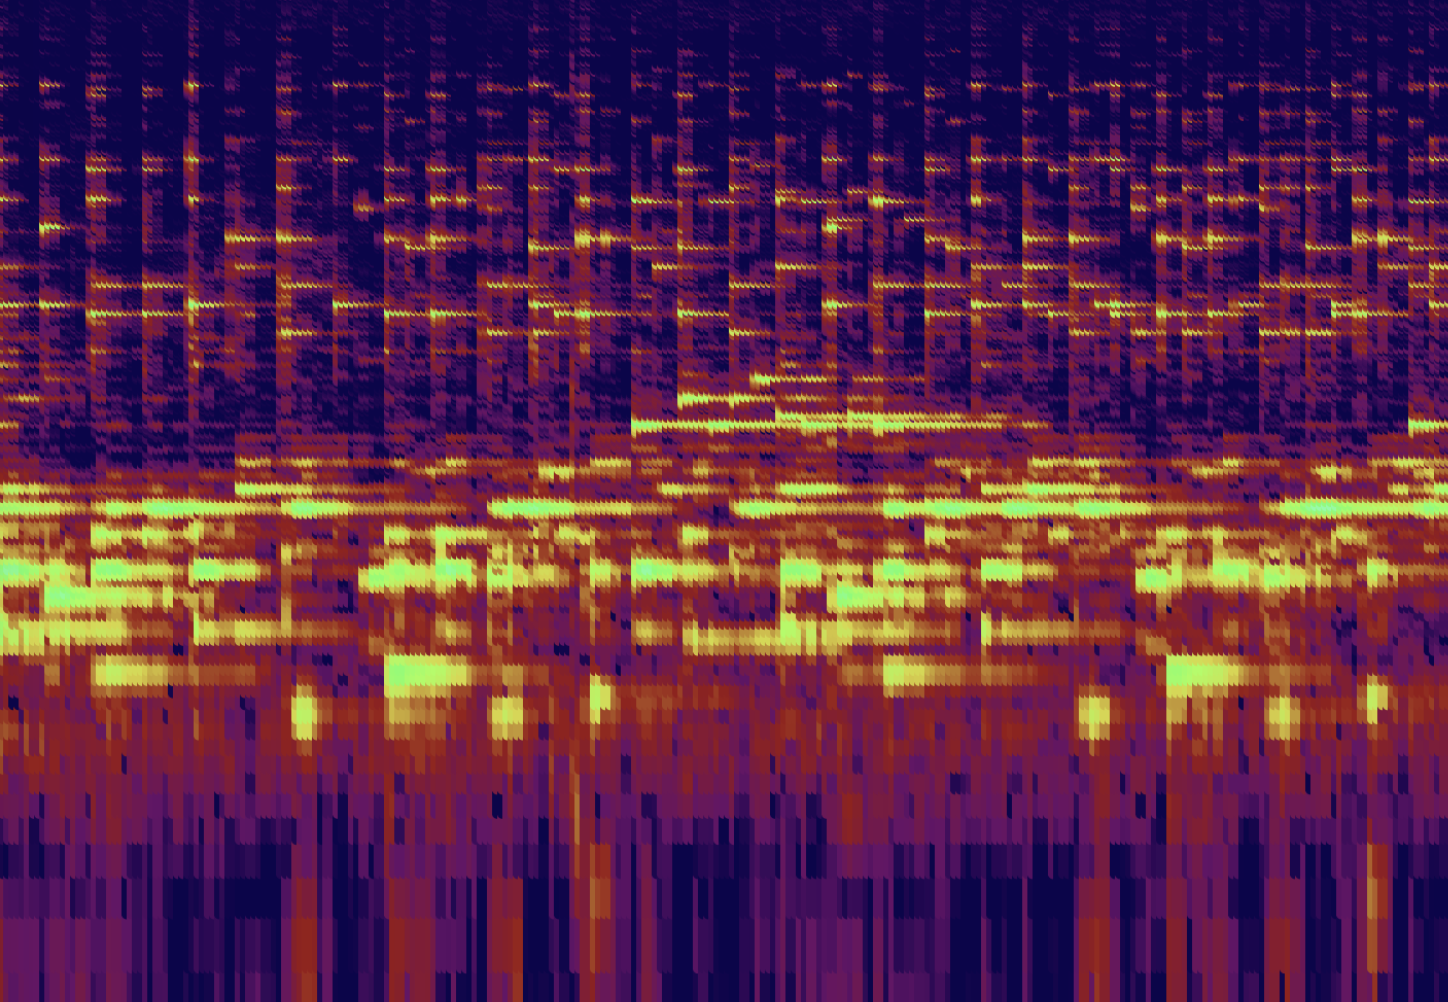
\includegraphics[width=0.45\textwidth]{SpectrumOfSound_2}
\caption*{Sonogram of part of Pachelbel's canon.}
\end{wrapfigure}

For practical applications, there is a useful algorithm called the Fast Fourier Transform (FFT), that substitutes the abstract mathematical formula. This allows us to make extremely fast computations and analyze signals in real time. Today many electronic ways of working with music are based on FFT. It forms the first step of extracting a score from a piece of played music. It can be used for instance for the automatic transcription of Jazz soli. It is also the basis of modifying music. The common practice of pitch adjustment in pop music (auto-tune) can be basically described as an ``analyze - correct - synthesis'' procedure. Special sound effects like letting an instrument speak like a human voice rely on automatic sound analysis of the involved spectra. Also automatic music recognition services like Shazam heavily rely on the fingerprint of a tune resembled by its sonogram.

The second screen of the exhibit displays a spectrum analyzer connected to the microphone input. On the left you have the spectrum, i.e. the instantaneous analysis of frequencies (Fourier transform) of the playing signal. At the right the spectrum leaves a trace to visualize the history of the input signal (sonogram). 

\begin{figure}[h]
\centering
\begin{subfigure}{0.45\textwidth}
\centering
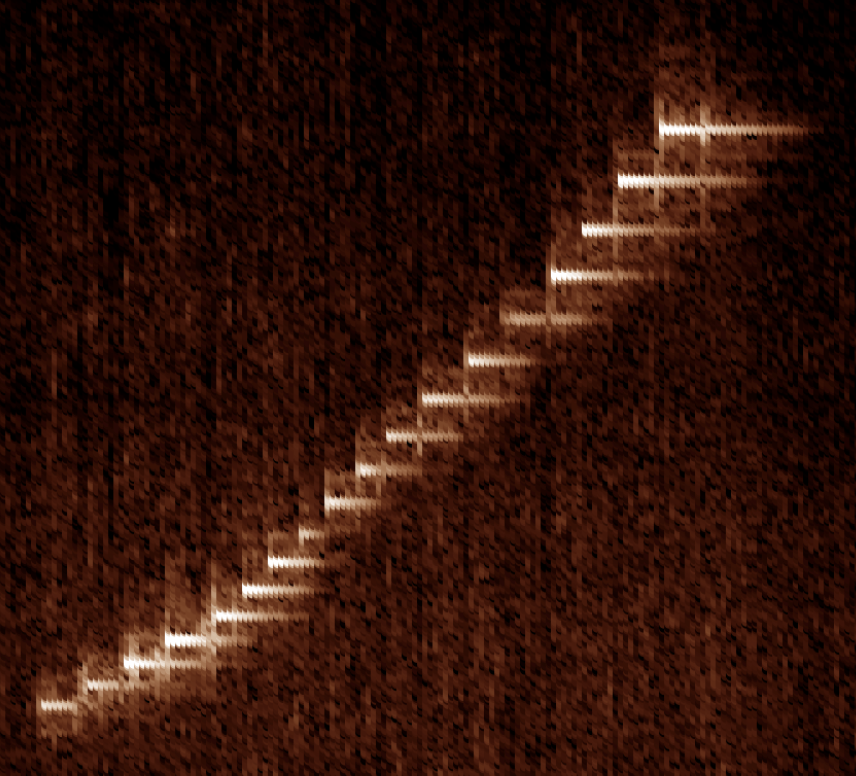
\includegraphics[height=3cm]{SpectrumOfSound_7}
\subcaption*{Chromatic scale linear.}
\end{subfigure}
\begin{subfigure}{0.45\textwidth}
\centering
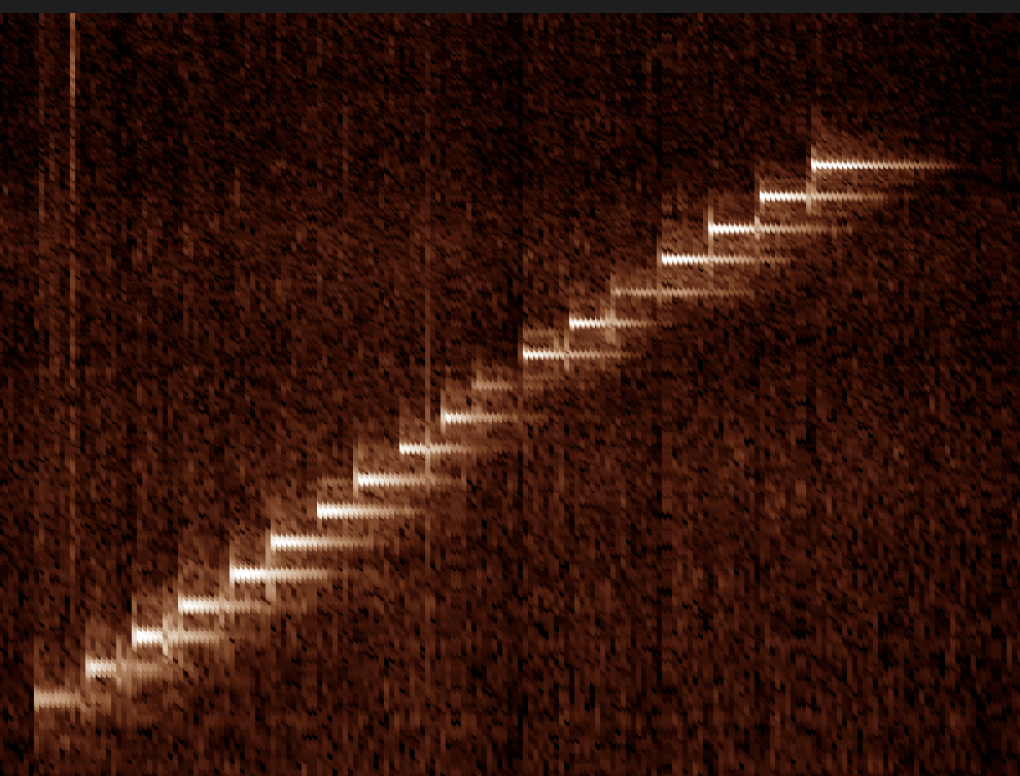
\includegraphics[height=3cm]{SpectrumOfSound_8}
\subcaption*{Chromatic scale logarithmic.}
\end{subfigure}
\end{figure}

Linear scale is best suited for sounds and overtones (frequencies $f$, $2f$, $3f$, $4f$, $5f$, ...), while logarithmic scale is best suited for musical tones (frequencies $f$, $af$, $a^2 f$, $a^2 f$, $a^2 f$, ...). Use the microphone to analyze your voice or the available instruments. Sing something, make noises, talk, or use the synthesizer to generate a tone. Put the microphone next to the speaker and analyze the sound produced. Try to identify the frequencies, their intensities, when they appear, when they fade out.


\begin{figure}[h]
\centering
\begin{subfigure}{0.45\textwidth}
\centering
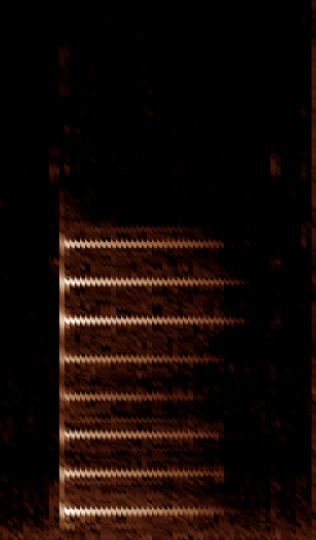
\includegraphics[height=3cm]{SpectrumOfSound_5}
\caption*{Overtones linear.}
\end{subfigure}
\begin{subfigure}{0.45\textwidth}
\centering
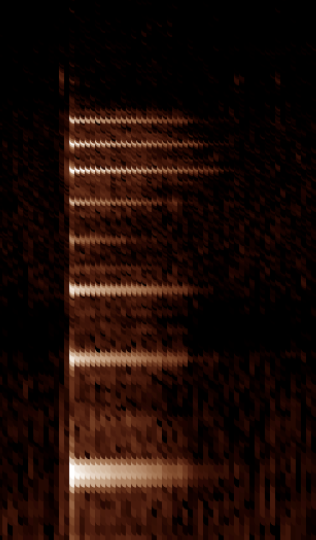
\includegraphics[height=3cm]{SpectrumOfSound_6}
\caption*{Overtones logarithmic.}
\end{subfigure}
\end{figure}


\vfill

Authors of this exhibit: \\ 
Synthesiser: Tero Parviainen, Eric Londaits (IMAGINARY). \\
Analyser: Jürgen Richter-Gebert (TU Munich). \\
Text: Daniel Ramos (IMAGINARY).


\section{Scale Lab}
We can hear a wide range of frequencies. Usually we don't use all the audible frequencies to make music, we select a discrete set of them to determine the pitch of each tone, and we call this set of frequencies a scale. Depending on the choice of the scale, we will be able to play some combinations. Interestingly, humans find that some pairs of frequencies sound ``good'' together (consonant), while others sound ``bad'' (dissonant). This is a physiological and psychological phenomenon still under debate and being actively researched today. This preference has determined the choice of scales and the practice of music since the beginning of its history.

In this exhibit, we explore the creation of scales and their properties. Along the gray horizontal line all the frequencies are represented. The markers represent frequencies selected for the particular  scale, and they are connected to the keyboard by the blue lines that allows us to play them. 

\begin{figure}[h]
\centering
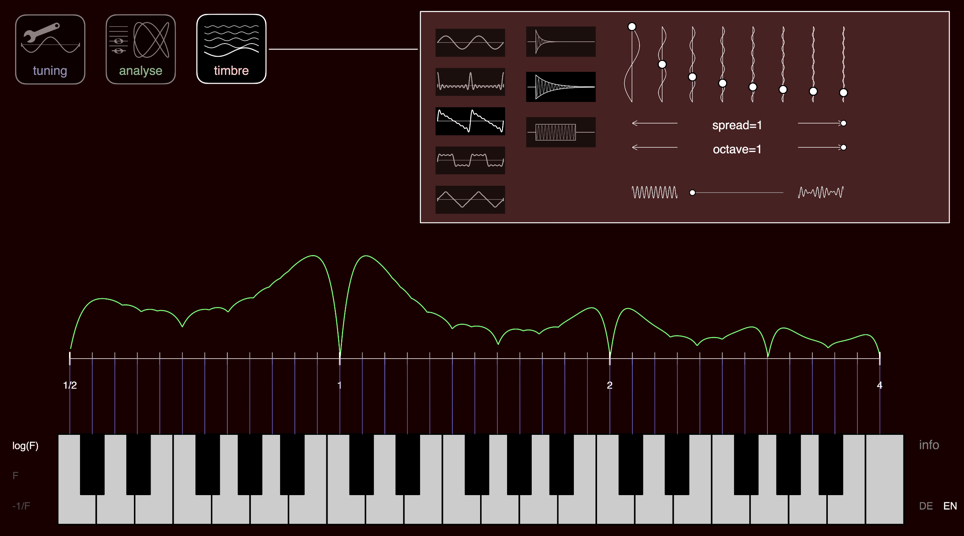
\includegraphics[width=0.9\textwidth]{ScaleLab_1}
\end{figure}

\subsection{The Tools}
A set of three toolboxes helps us influence the characteristics of a tone (timbre), the selection of the pitches for the scale (tuning) and to analyze properties of tones and combinations of tones (analyze).

\subsubsection{Tuning}
You can choose Western scales (with different tunings), two oriental scales (Raga, Gamelan), and two tools to generate scales (one with a step-generator and another with free pointing).

\subsubsection{Analyze}
The analyze toolbox contains the implements that help you to understand the scale/tuning you selected.

\subsubsection{Waveform}
This is the signal you hear, the movement of the speaker's membrane (and your eardrum) over time. Choose a sine as timbre and press one key to hear a pure frequency. Play two or more to see the combined waves (addition). Choose a different timbre (composed of many frequencies) to see its waveform and hear the difference.

\subsubsection{Lissajous} 
This curve is drawn by a moving point with an x-coordinate given by the oscillation determined by the first key stroke, and a y-coordinate given by the second key stroke. This works better with a pure sine waveform as timbre, but it also creates very interesting curves for more complicated timbres. Simple ratios between the two frequencies give simpler figures, which are also the more ``consonant''.

\subsubsection{Ratio}
You can see the proportions between the (fundamental) frequencies of the notes played. Check the different scales to see how simpler ratios are related to consonant intervals.

\subsubsection{Dissonance curve}
Real instruments don't produce a single frequency, instead many of them simultaneously (spectrum). Thus consonance or dissonance depends on the interaction of the two groups of frequencies. This curve (based on a concept from Helmholtz) attempts to measure dissonance (badness) of every tone with respect to the fixed middle C tone, and it varies when the timbre is changed. Note that dissonance is at a minimum for an octave jump or fifth and major third jumps.

\subsubsection{Timbre}
A musical tone produced by an instrument is not usually a single pure frequency, but a mixture of different frequencies with different intensities (spectrum). This toolbox allows the selection of  some predefined spectra as well as defining one yourself by adjusting the sliders. All scales, tuning settings, and analysis performed with other toolboxes is strongly affected by the timbre of the instrument you choose to play.

\subsection{Backgrounds and Experiments}
The following pages describe concepts and experiments that can be experienced using the Scale Lab exhibit.

\subsubsection{Beating}
If two frequencies are close, an exciting and fundamental acoustic phenomenon occurs: the sound seems to periodically increase and decrease in volume... and it actually does. There are two ways to explain this effect. One is more qualitative: assum
e you have two frequencies one of 100 vibrations per second and one of 101 vibrations per second. At every moment of time these two waves will sum up. If the trough of one wave meets the peak of the other the two signals will cancel out. If a peak meets another peak the intensity is double that of the single signal. 

\begin{figure}[h]
\centering
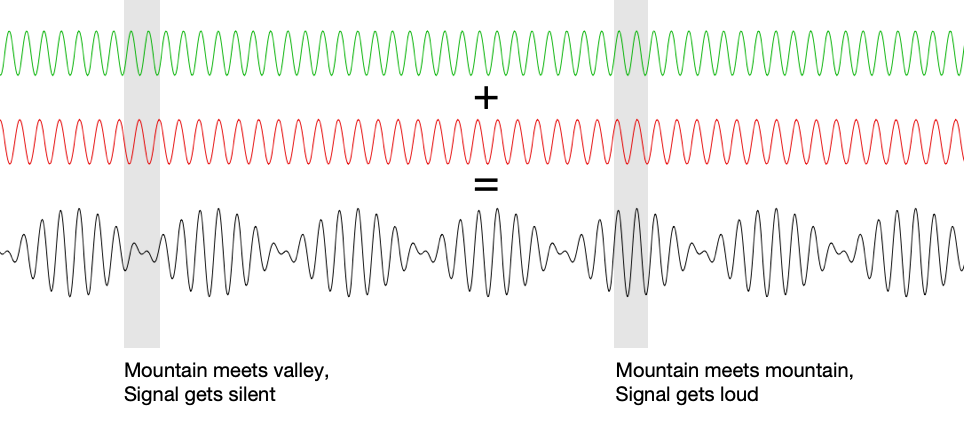
\includegraphics[width=0.9\textwidth]{ScaleLab_3}
\end{figure}

The second way to think about it is more quantitative. There is a nice trigonometric formula that describes what happens if two sine waves of different frequencies $f_1$ and $f_2$ are added: 
$$\sin(f_1 \cdot t) + \sin(f_2\cdot t) = 2 \sin\left( \frac{f_1+f_2}{2}\cdot t\right) \cdot \cos\left( \frac{f_1-f_2}{2}\cdot t\right) .$$
The resulting wave can be considered as a signal vibrating in the average frequency (the sin part of the right hand equation) and modulated by a low frequency signal depending on the difference of the frequencies (the cos part of the right hand equation). If the frequencies are close together this will be heard as low frequencies change in intensity.

\paragraph{Experiment:} Go to timbre and select a pure sine wave. Then use multi-touch on the central horizontal frequency line to create two nearby tones by using two fingers. Listen to the beating. The closer the frequencies are the slower the beating. If you move them far apart at some point the beating gets so fast that you perceive it as a rough dissonance. Moving them even further apart they will be perceived as two different tones. Analyze this using Lissajous or wave to actually see the beating.

\paragraph{Music:} Slow beating sounds like a bit like a vibrato, it makes a tone sound richer and a bit more organic. This is the reason why in several instruments beating is taken as part of the sound generation process. In a piano the high frequency notes usually have two or three strings. These strings are slightly detuned with respect to each other, resulting in an organic and rich tone. Also a Musette register on an accordion has two slightly detuned vibrating metal tongues generating a vibrato sound.

\subsubsection{Sound from Overtones}
The timbre settings of Scale Lab allow for much more than just simple sine waves, you can combine sine waves to generate a complex sound. The sliders in the timbre box allow you to add multiples of the base frequency. If the spread slider is set to 1 these are really the integer multiples $f$, $2f$, $3f$, $4f$, $5f$, $6f$, $7f$, $8f$. of the base frequency. Fourier synthesis implies that any periodic signal can be generated by a weighted sum of sine waves of the above type. You would need infinite summands to replicate a perfect signal, but the eight frequencies offered by Scale Lab are already pretty precise. 

\begin{figure}
\centering

\includegraphics[width=0.9\textwidth]{ScaleLab_5}
\caption*{This illustrates how the summation of overtones with intensity 1, 1/2, 1/3, 1/4, ... results in a sawtooth-like periodic function.}
\end{figure}

\paragraph{Experiment:}
Go to timbre and experiment with the different presets for wave forms (buttons on the left). Move the individual sliders of the timbre overtones to monitor how the sound changes. Use the ``analyze tool'' to see the shapes of the waves you generated.

\paragraph{Music:}
As a matter of fact, the sound of many instruments (in particular strings, brass or woodwind instruments is nicely approximated by decomposing the sound into a composition of overtones. This has to do with the specific physics of the instruments. 

\begin{figure}
\centering

\includegraphics[width=0.9\textwidth]{ScaleLab_6}
\caption*{The image shows the partial waves of an ideal vibrating string. They correspond exactly to the overtones, resulting in a sound that can be very well modeled by this approach.}
\end{figure}


\subsubsection{Spread partials}
The world is not an ideal laboratory. Physics is dirty and sounds are not perfect sums of overtones. As a matter of fact, most instruments create sounds where frequencies of the higher vibrations do not perfectly match overtones. For instance the fact that a string is not infinitely thin results in a certain spread of the overtones. The thicker the vibrating material gets the more extreme is the deviation form the ideal overtone series. The spectrum of a church bell is substantially different from an overtone series. This is not a bad thing. It makes sounds richer, more individual, or more characteristic. Below you see what happens if the overtone spectrum is replaced by a spread spectrum where the frequencies follow the law 
$$1^af, 2^af, 3^af, 4^af, 5^af, 6^af, 7^af, 8^af$$
for a small exponent $a$. Observe that the resulting sum of the partials (this is the correct name here) shows ever changing behavior in the resulting sound curve and is no longer periodic. The resulting sound is rich and organic. 

\paragraph{Experiment:} 
In the  Scale Lab Timbre Box there is a slider called spread right under the overtone sliders. Play with the slider to experiment with spread and compressed spectra. Listen how the sound changes even if you only add a very slight spread. Analyze the resulting sound with the wave tool to see how the wave forms change. How do intervals sound? What is the difference between a small and a large spread? Between a spreading and a compression of the spectrum? There is a whole world to be discovered.


\subsubsection{Dissonance curves}
As soon as two tones (with a certain spectrum of partials) are played together our brain starts to categorize the intervals in a range
A between pleasant sounding (consonant) and not-so-nice sounding (dissonant). One can think of the entire art of music as the art of creating the right tension between consonance (to please people) and dissonance (to make it interesting). Different epochs and cultures have different opinions at what is good style, but the global topic remains.

\begin{figure}[h]
\centering

\includegraphics[width=0.9\textwidth]{ScaleLab_7}
\caption*{There is another interpretation of the richness of sound that arises. Since the partials do not perfectly match the overtones as soon as intervals are played, there is a substantial and quite irregular beating of the higher frequencies.}
\end{figure}

Already around 1870 Hermann von Helmholtz developed a mathematical theory of consonance and dissonance. The idea behind it is brilliant and simple. Since whenever two tones are played together many partials sound at the same time, one has to sum up the dissonances between all pairs of involved sine waves to get the dissonance of the entire sound. Therefore, he reduces the question of dissonance of complex sounds to the question of dissonance between sine waves. (One might ask if this is a reasonable assumption but at least it is a good starting point). However, what is the dissonance between two sine waves? Here we need empirical data. It turns out that if sine waves with more or less of identical frequency are not perceived as dissonant. A small, low frequency beat even slightly pleases. However, as soon as the beating becomes too fast it is perceived as rough and dissonant. This effect is particularly strong for beats between 10 and 25 beats per second, after that the effect decreases again. If the tones are too far apart they are just heard as two sine waves. Below you see a dissonance curve of a sine wave referring to a middle C.

\begin{figure}[h]
\centering
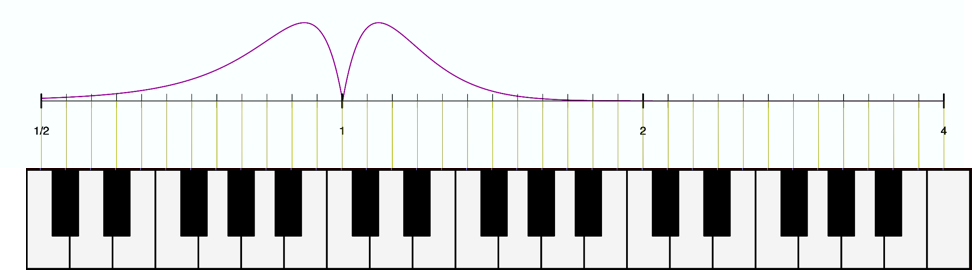
\includegraphics[width=0.9\textwidth]{ScaleLab_9}
\end{figure}

Things get interesting as soon as the spectra become complicated. The next picture shows the dissonance curve resulting from a rich overtone spectrum. Dissonances between overtones of the two tones generate characteristic maxima and minima of that curves. Notice that for the usual perfect overtones you get minima at the octave, the fifth, the quarter and the third. 

\begin{figure}[h]
\centering
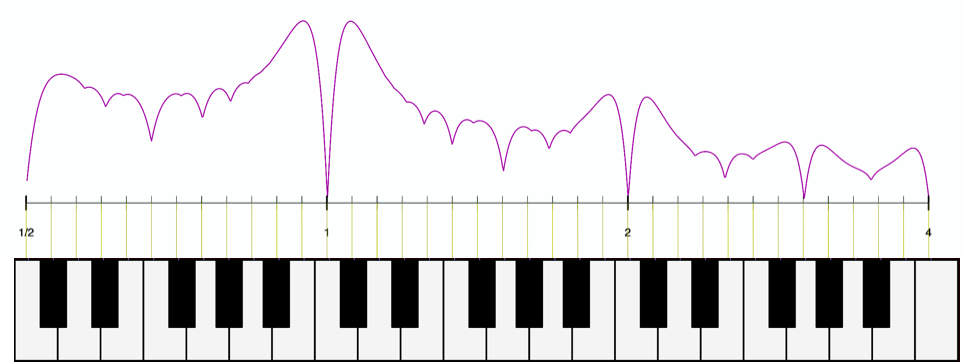
\includegraphics[width=0.9\textwidth]{ScaleLab_10}
\end{figure}

\paragraph{Experiment:}
Start the dissonance curve analyzer and play intervals with the central C. Play with different timbres and experiment with different intervals, Does the prediction meet you personal perception?


\subsubsection{Dissonance and spread partials}
What happens if we study the dissonance behavior of a spectrum with spread partials? The dissonance behavior is very much determined by the dissonance between the overtones or partials. Consequently, as soon as the partials are ``out of place'' you get a new dissonance behavior.

The following image shows what happens to a slightly spread spectrum ($a=1.08$):

\begin{figure}[h]
\centering
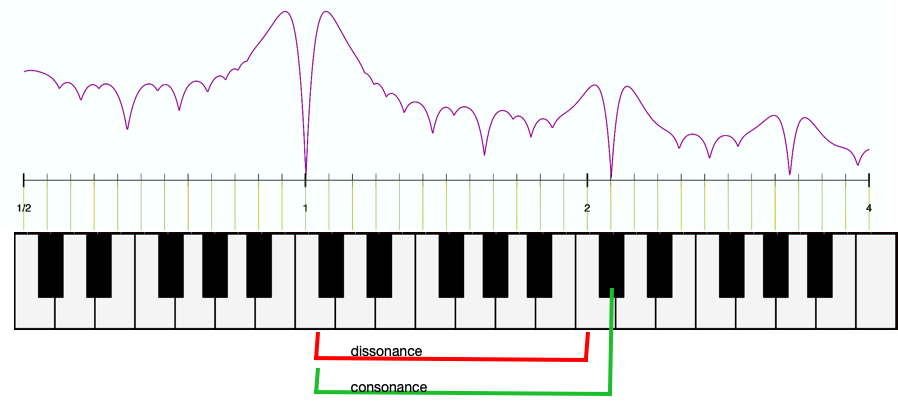
\includegraphics[width=0.9\textwidth]{ScaleLab_11}
\end{figure}


For a musician used to our classical tone system the result might be a little bit shocking. Suddenly intervals that usually sound consonant (like the octave) sound heavily dissonant. While others that usually sound very dissonant (like the small ninth between C and c\#) sound as sweet as sugar.

Therefore, instruments that generate a spread or compressed spectrum require a different kind of scale. Or to put it differently, our Western tonal system is heavily influenced by the fact that we have strings, brass and woodwinds.

There is an amazing cure to fix the dissonant sounding octaves: Spread the frequencies of your scale as well! After that an octave is no longer an octave, but it sounds like one.

\begin{figure}[h]
\centering
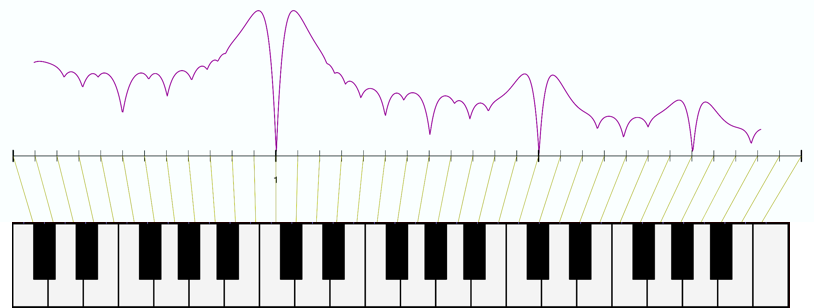
\includegraphics[width=0.9\textwidth]{ScaleLab_12}
\end{figure}

\paragraph{Experiment:}
The following experiments may be eye-opening. Start the dissonance curve analyzer and play intervals with the central C. Experiment with the spread of the spectrum and with the spread of the octave. Spreading both by the same amount gets you close to the usual tonal experience.

\paragraph{Music:}
In some instances, it may be good practice to spread scales. If you design the bells for a church tower adapting the scale to a spectrum is a good idea. Even an ordinary piano sounds more brilliant if the octaves are slightly spread. However, a piano with slightly spread scales will make it difficult to play along with other instruments. Music is full of compromises.

\subsubsection{Western Tuning Systems}
We have seen that the timbre and the frequencies of the partials heavily influence the dissonance behavior of intervals. As a consequence, the selection of pitches (the scale) used on an instrument should depend on the sound characteristics of the instrument. Western culture instruments (harps, pianos, flutes, trumpets, have a close to perfect spectrum in the sense that the partials are very close to the theoretical overtones. Therefore, frequency ratios of $2 : 1$ (octave), $3 : 2$ (fifth), $4 : 3$ (fourth), $4 : 5$ (major third) and $6 : 5$ (minor third) result in relatively consonant intervals (in this order with decreasing strength). 

It turns out that fifths, fourths (Gregorian music), then later thirds (baroque) and even later more dissonant intervals (impressionists, expressionists) entered the musical language in the Western culture. 

What is a good selection of pitches for such music? What are good scales? Answering these questions in depth could easily fill a one year university class. We will only scratch the surface. 


12-Tone system: Current Western music culture systems of twelve tones within an octave are predominant. The reason for this is in a sense mathematical. Stacking 12 perfect fifths nearly hits stacking seven octaves. Or in formulas:
$$\left( \frac{3}{2}\right)^{12} = 129.7463 \ldots \approx 2^7 = 128 .$$
The 12 steps are the first time this stacking procedure comes close to an octave relation. If one wants a tonal system that is focused around octaves and fifth, then 12 tones are a good start.

Unfortunately, this relation is not perfect and this is where the entire story of tuning systems begins: one has to make compromises and different epochs resolved this tension in different ways.

\begin{figure}[h]
\centering
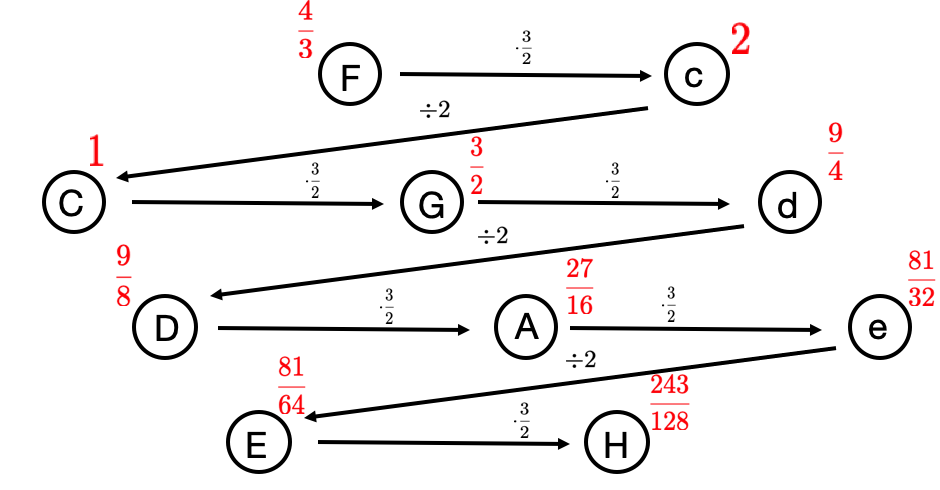
\includegraphics[width=0.7\textwidth]{ScaleLab_14}
\caption*{Pythagorean tuning}
\end{figure}


Pythagorean Tuning: Let us start with Pythagorean tuning, which focuses around the idea of having as many perfect fifths as possible. Focus on the seven tones of our C major scale and see what happens. We label the tones by frequency ratios with respect to C and divide by two (drop an octave) every time we become greater than two. The following diagram shows the frequency ratios of notes in the Pythagorean scale and how they are derived. 

All fifths and octaves in this tuning are perfect. However, notice that the note E gets assigned a frequency value of 81/64. This is not a perfectly tuned major third, the perfect third would be $5/4=80/64$. 

Thus the Pythagorean third is off by a factor of 81/80 from the perfectly tuned third. Most likely the Pythagoreans would not have cared a lot since thirds only became an important interval in music over 1500 years later. As mentioned above not all the fifths can be perfect. If 11 fifths are perfectly tuned the last one must sound really terrible.

\begin{figure}[h]
\centering
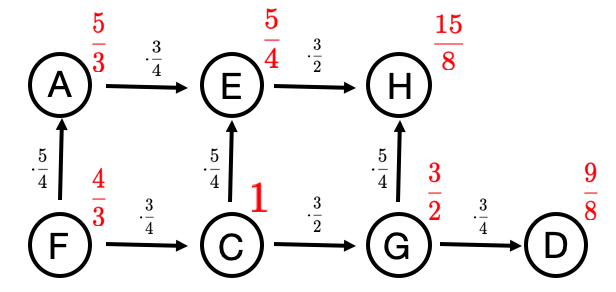
\includegraphics[width=0.7\textwidth]{ScaleLab_15}
\caption*{Just tuning}
\end{figure}

Just Tuning: Let us now consider a tuning that focuses on fifths and thirds. It is called just tuning. For the seven notes in the C major scale it uses the following tuning pattern. 

You can play many perfect thirds and fifth with this tuning, but you loose some others. As a matter of fact, this little grid is a small portion of the Tonnetz.


Equal tempered tuning: If you extend both the Pythagorean and the just tuning to all 12 halftones. Some intervals will be perfect, but others won't sound as perfect. The modern approach taken to tuning is to avoid this by equally spreading the error over all intervals. (This might be considered as a kind of democratic approach to tuning). In equal tempered tuning an octave is simply split into 12 equal steps. Each halftone step multiplies the frequency by a factor of $\sqrt[12]{2}$ , which reaches a perfect octave after 12 steps. Using this method, all fifths carry the same error. The same happens for chords and for all other intervals. Let us compare the values of equal tempered tuning to perfect tunings,
$$\textrm{for fifth: } (\sqrt[12]{2})^7 = 1.498\ldots \approx 1.5 = \frac{3}{2} ,$$
$$\textrm{for thirds: } (\sqrt[12]{2})^4 = 1.26\ldots \approx 1.25 = \frac{5}{4} .$$
Note that these approximations are very good.

\paragraph{Experiment:}
Open the tuning box and experiment with different Western tunings. The colors shown in the Tonnetz indicate how close an interval is to a perfect one. It is also very instructive to analyze the different tunings with the ratio tool. It shows the ratios of intervals if they are played on the keyboard. The picture below shows the frequency ratios for a major C chord.

\begin{figure}[h]
\centering
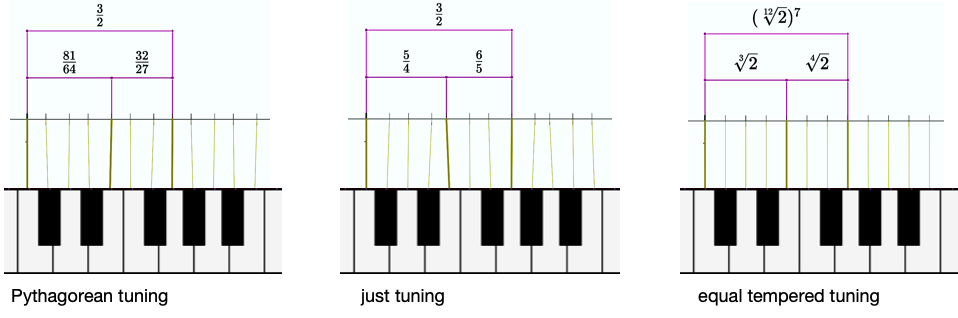
\includegraphics[width=0.95\textwidth]{ScaleLab_18}
\end{figure}

\subsubsection{Indian Raga Scales}
There is another way of playing many perfect fifths and thirds: Add more tones to the scale!  The tuning system for Indian Raga music make utilizes this approach. In short, these tuning systems can be characterized by the following tuning scheme. 

\begin{figure}[h]
\centering
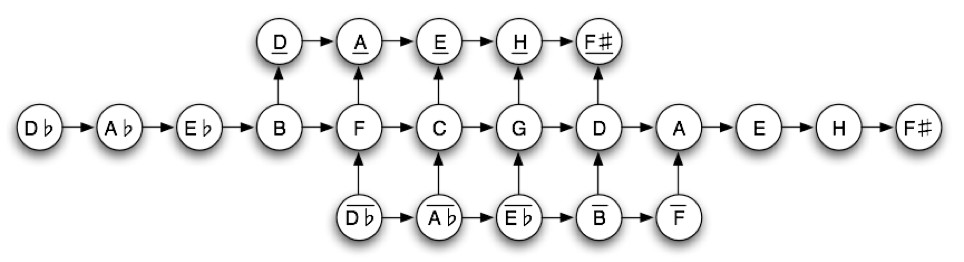
\includegraphics[width=0.9\textwidth]{ScaleLab_19}
\end{figure}


Every horizontal arrow indicates (up to octave jumps) a perfect fifth and every vertical arrow a perfect third. Unlike Western music, Raga music has more an oral than a written tradition. Hence, it is a little difficult to nail down a concrete tuning system but the one described above consisting of 22 tones is accepted among people who analyzed Indian music. What is so special and interesting about this tuning system and why are there exactly 22 tones? 

First of all, it should be noted that Indian Ragas always refer to a given base tone. Usually a drone interval is constantly played in the background, the usual one is a C-G sound. Observe how the middle between the C and G is the symmetry center of the above diagram.

The central row of the diagram is the Pythagorean scale with 11 perfect fifths. Now we saturate it by adding perfect thirds, which is done in a very clever way. To see this we reorder the notes of the Pythagorean scale to form a chain of halftones. We get:

\begin{figure}[h]
\centering
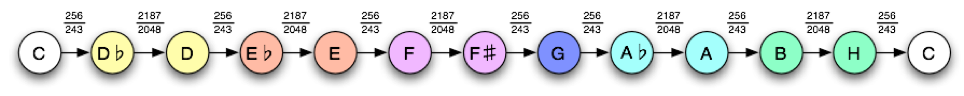
\includegraphics[width=0.95\textwidth]{ScaleLab_21}
\end{figure}

The ratios between the tones represent the frequency ratios that come from the Pythagorean tuning. 

You can see that, almost magically, only two kinds of fractions occur. The coloring in the diagram marks the bigger of the two fractions, thus we have big halftone steps and small halftone steps. Two tones that are related by a big step have the same color. Now one can split the interval of 2187/2048 in an elegant way by introducing two new notes. 

\begin{figure}[h]
\centering
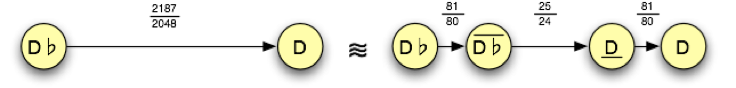
\includegraphics[width=0.95\textwidth]{ScaleLab_22}
\end{figure}

In the example above you additionally get a higher version of the $D\flat$   and a lower version of the $D$. These are exactly the two versions added in the above tone system. We can now do a similar split for all other big halftone steps. This results in the system with 22 tones, shown in the following colored version of this tone system:

\begin{figure}[h]
\centering
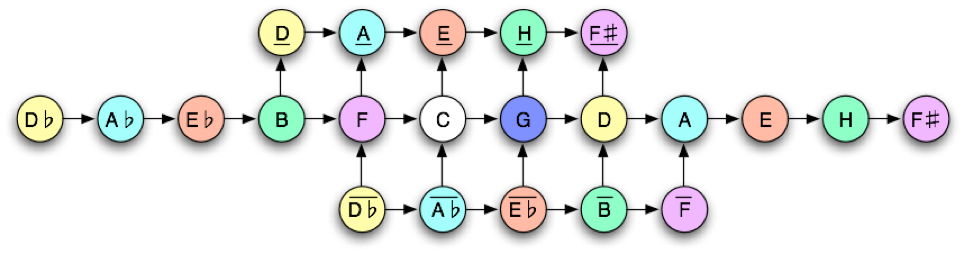
\includegraphics[width=0.95\textwidth]{ScaleLab_20}
\end{figure}

Notice that the C and G play a special role in this system as the only notes that are not involved in a split interval.

The tones of the Raga tuning system are called Shrutis. As in the Western tuning systems, often a melody does not make use of all tones at the same time. Instead, certain notes are selected to form smaller scales based on the bigger tone system. Also the selection of sub scales (usually of four to seven tones) follows certain rules. But we will not go into those details here.

\paragraph{Experiment:} Open the tuning box and experiment with the sounds of the Raga tunings. You can start the drone tone and select among plenty of commonly used sub scales of the 22 tone system. It might also be interesting to measure frequency ratios between the tones.

\vfill

Author of this exhibit: Jürgen Richter-Gebert, Technical University of Munich / Sound Engine: Patrick Wilson and Aaron Montag / based on CindyJS.org
Text: Jürgen Richter-Gebert (TU Munich)



\section{Tonnetz}

The musical scale we use in Western music tradition is a choice of tones, that is, a selection of frequencies that we use to tune an instrument to make music.

How do we name the notes? How do we represent these notes graphically? Which notation do we use to describe them on a score or to build an instrument? The first obvious choice would be to order them by pitch and name them sequentially. However, this doesn't reflect their relationships or their respective roles in musical language.

By playing together a first note and a second one with double the frequency (ratio 1:2), the result is so consonant and the two tones mix together so well that we have the impression that they are the ``same'' note. In fact we even call them by the same name. In this case, the interval between two such notes is called an ``octave''. In modern tuning (the equal tempered system of the piano), an octave is divided into 12 equal parts and these equal parts correspond to the 12 notes of the chromatic scale.

But we don't use all these 12 notes equally, some are used more often, at least historically, when the notation was developed in the Middle Age. This is why we have the ``main'' notes in a scale representing the white keys of the piano (C, D, E, F, G, A, B), called the diatonic scale, and ``secondary'' notes that we describe as alterations of a main note with flat and sharp (such as $C\sharp$ or $E\flat$) are represented by the black keys.

Thus there are seven main notes in an octave, and the eighth has the same name as the first one (hence the term octave).

Ordering the notes by pitch, like in the piano keyboard, may be reasonable; but it does not reflect all the relationships between notes. 

Because of the octave relation, it makes sense to represent notes in a circle, the so called Chromatic circle. The notes are

C, C\#, D, D\#, E, F, F\#, G, G\#, A, A\#, B

and after the last note of the scale (B), the first note (C) follows. In modern tuning, the intervals are all equal (called semitone) and sharp and flat coincide as in $C\sharp = D\flat$. This relation is called the enharmonic identification. 

Another fundamental relation is the Fifth (or more precisely the perfect Fifth). This is the interval between C and G or between F and C, and it corresponds to adding 7 semitones to an initial note. It is called a fifth because in the 7 notes scale, if C is the first note, G is the fifth one. After the octave, it is considered as the most consonant interval, as one can experience by playing the two notes together. Thus, it makes sense to have them close as in the Circle of fifths, which is built by listing the notes in steps of 7 semitones: 

C, G, D, A, E, B, Gb, Db, Ab, Eb, Bb, F

Same as before, the F is followed by the C.

This representation is very useful to musicians because the notes that match well are closer together. This also explains why the white keys of the piano, represented by the  notes A,B,C,D,E,F,G, are the ``main'' ones (with respect to the ``secondary'' ones): if you start at F, you can repeat the fifth interval six times and this will give you a chain of seven notes corresponding precisely to the diatonic scale. The note ``C'' is the first one in Latin notation (Do, Re, Mi, Fa, Sol, La, Si), in what is called the ``major mode'', but if you start the scale in A, like in the English notation, you obtain the ``minor mode''.

Two other very consonant relations are the Major Third (adding 4 semitones) and the Minor Third (adding 3 semitones). For instance between C and E there is a Major Third (E is the 3rd note on the scale). Between C and Eb, or between D and F there is a Minor Third (they are only 3 semitones apart).

When notes are played together, we obtain what is called a chord. The most common chords are triads (when 3 notes are played together) and the basic recipe to build a Major chord is to pick one note x (tonic) then add its Major Third and Fifth. This gives you three notes (x, x+4, x+7) that sound very pleasant and bright. For instance C - E - G is the C-Major chord. Analogously, Minor chords are created by the tonic x then adding its Minor third and Fifth, to obtain (x, x+3, x+7), that sound more sad and dark. For instance, C - Eb - G is the C-Minor chord.

There is a graphical representation of notes that reflects some of these relations. It goes back to mathematician Leonhard Euler, and it is known today as the Tonnetz (German for "network of tones"). The classical tonnetz (labeled here as 3,4,5) consists of a triangular grid where each vertex is associated to a note (up to an octave). There are three lines or directions in the triangular grid. In one direction notes are rising in fifths, in another in major thirds and in the final one in minor thirds. This is possible because raising 7 semitones in one direction corresponds to raising 4 semitones and 3 semitones in the two other edges of each triangle. The three notes form a triangle in the Chromatic circle with arc-sides 3, 4 and 5, which is the label we use for this tonnetz.

With this diagram, all pairs of notes separated by a fifth, major third or minor third are adjacent. Furthermore, all major and minor chords are represented as the triangular faces of this diagram. 

There are other types of triads, depending on the intervals between their notes. For instance Augmented chords are (x, x+4, x+8), which form a triangle with sides 4,4,4 in the chromatic circle (or in the fifth circle). We can build a tonnetz that represents these chords using these intervals as increasing steps in each direction. Any three numbers a,b,c, that add up to 12 represent a triangle on the chromatic circle and can be represented in a tonnetz. Using combinatorics, there are 12 possible ways of choosing 3 numbers a,b,c between 1 and 12, so that a+b+c=12. These are the 12 possible tonnetze.

On the diagram we can also see the dual graphs of the tonnetz. A dual graph is built by replacing each face by a vertex, each vertex by a face, and connected vertices by adjacent faces. This diagram has the same information as the original one, but now each triad is a vertex of an hexagonal tiling and each note is a face (an hexagon).

The tonnetz representation contains a lot of musical information. For instance, adjacent triangles represent triads that have two tones in common, and thus it is a natural chord progression in composition to go from one to another.

Finally, these graphical representations can be used to transform a piece. The most basic transformation is pitch shifting, just adding a fixed amount of semitones to all notes in a music piece. This is usual to adapt a piece for a singer's range of voice. Geometrically it corresponds to a translation in the piano, but the white-black keys do not match. Better it is to consider a rotation on the chromatic circle, then all the notes are just rotated, or a translation in the tonnetz.

An example of such a transformation would be a rotation on the Circle of fifths. That is just jumping 7 semitones at once (since a fifth is equal to 7 semitones). Again, if we have the piece represented on a tonnetz, that corresponds to a translation of the net in any of the directions.

A more interesting transformation is a rotation of the tonnetz. Consider one piece represented in the tonnetz. Fix one note (for instance the first note on the piece), and then switch all the rest of the notes by their counterpart after rotating 180 degrees on the tonnetz. This transformation is called a ``negative harmony'' and transforms every major chord into minor chords and vice-versa. You can hear an example on the exhibit, by selecting the classical 3,4,5 tonnetz.

\vfill

Authors of this exhibit: Moreno Andreatta and Corentin Guichaoua (SMIR Project). Supported by CNRS/IRCAM/Sorbonne University, USIAS (University of Strasbourg Institute for Advanced Study), IRMA/University of Strasbourg. Adapted by Philipp Legner. Text: Daniel Ramos (IMAGINARY)


\section{Beat Box}
Along with melody and harmony, rhythm is one of the most important components of music. The exhibit ``Beat Box'' explores various ways to create and analyze rhythms by mathematical methods.

\subsection{Fibonacci Rhythm / Hemachendra (Fibonacci) numbers and 2-1 rhythms}
It only seldom happens in science that important concepts are named after the person who dealt with them first. This is also the case for the famous Fibonacci numbers. Fibonacci mentioned them in the context of a calculation exercise in his book Liber Abaci published in 1202. As a matter of fact already much earlier in 1050 these numbers were studied by the Indian scholar Hemachendra in a very interesting context related to rhythm.

\begin{wrapfigure}{l}{0.4\textwidth}
\centering
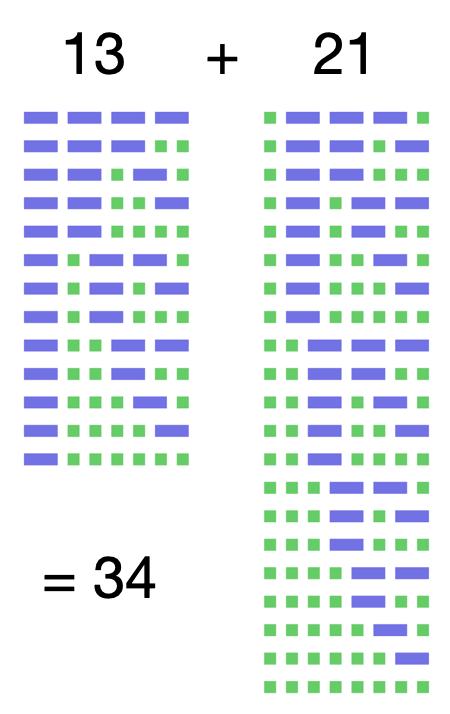
\includegraphics[width=0.4\textwidth]{BeatBox_1}
\caption*{Fibonacci rhythm}
\end{wrapfigure}
Assume you want to fill a rhythm of n beats with patterns of either length 1 or of length 2. For instance an 8-beat rhythm could be filled by 1-1-1-1-1-1-1-1 or 2-2-2-2 or more complicated patterns like 2-1-2-1-2 or 2-1-2-2-1. How many possibilities are there? Such questions arise both in poetry when talking about verses and syllables, or in music when talking about rhythms built from quarters and halves. It turns out that the number of actual possibilities is a Fibonacci (or better Hemachendra ) number. A number from the sequence

1, 1, 2, 3, 5, 8, 13, 21, 34, 55, 89,144,...

where (after starting with 1, 1) each number is the sum of the preceding two. In fact there are exactly 34 ways to fill an eight beat pattern with 1s and 2s. 

\paragraph{The Music:}
To avoid repetitive patterns in music it is sometimes very good to be aware of all possibilities that satisfy a given requirement. The question of filling in beats with longs and shorts for instance has nice applications in the art of tabla playing. Here often the shorts and longs are not literally one note but fixed drumming patterns that fill either one or two beats. Using only two fixed patterns but being flexible with the macro rhythmic level of how to combine them creates a stylistic coherence while at the same time it creates richness. 

\paragraph{The Math:}
Why do Fibonacci numbers pop up in this context? Let us see how we can reduce the problem of filling 8 beats to the problems of filling 6 and 7 beats. Each eight beat rhythm either starts with a short or with a long note. If it starts with a long note there are as many ways to complete this as there are 7 beat patterns. If we start with a long  note then we have 6 beats to fill and there are as many possibilities as there are for 6 beats. Hence the number of 8 beat patterns equals the sum of the number of 7 beat and 6 beat patterns. Et voilà... the Fibonacci recursion. 

\paragraph{The Exhibit:} The exhibit is mainly an automatic tabla rhythm machine based on the above observations. Listen and enjoy! The sound samples for the fast Rhythm were, by the way, taken from a talk of Manjul Bhargava, a Fields Medalist, who also gave very inspiring talks on that topic, where he himself plays the tabla. 

\subsection{Clapping / Steve Reich's Clapping Music}
Want a challenge? Here it is! Try to clap along with one of the two voices in our Clapping exhibit. Or even better, find a partner and together clap both voices. For every position of the green point in the exhibit the challenge is different.

The piece you hear in the exhibit is an amazing example of how a simple idea can create interesting and complex musical patterns. Inspired by the clapping of Flamenco dancers, Steve Reich composed this amazing little piece of music. It consists of a simple 12-beat clapping pattern: 

\begin{figure}[h]
\centering

\includegraphics[width=0.9\textwidth]{BeatBox_2}
\end{figure}

3 claps - pause - 2 claps - pause - 1 clap - pause - 2 claps - pause ... repeat

The complexity is achieved by playing exactly the same rhythm with two players but shifting the beginning of the second player by n-beats for a chosen number n=0 to n=11. There are twelve possible such shifts each generating a different rhythm. Can you clap all of them with your partner?

\begin{wrapfigure}{l}{0.35\textwidth}
\centering
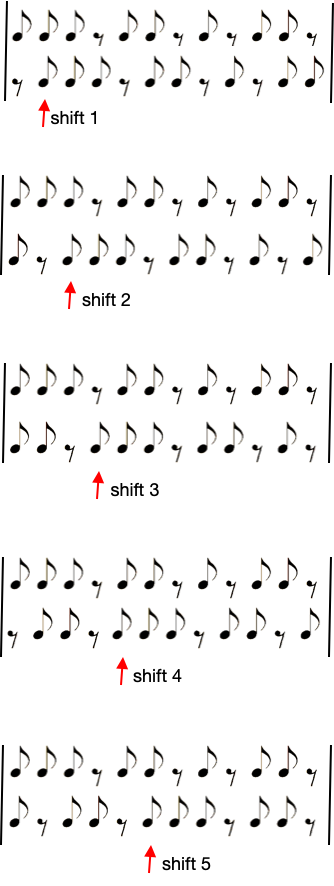
\includegraphics[width=0.35\textwidth]{BeatBox_3}
\end{wrapfigure}
\paragraph{The Music:}
A Minimal Music (mainly composed by Steve Reich) attempts to create interesting music by minimalistic progression of score. Shifting a rhythmical pattern by just one beat might be considered as a typical stylistic element of Minimal Music. In fact the clapping piece needs a tremendous concentration as soon as both parts are played together. Hence although it is minimal it is by no means easy.

\paragraph{The Math:} How many rhythmical patterns are suitable for creating a piece like Clapping Music. Let's stick to a 12 beat sequence. First of all there are altogether $2^{12} = 4096$ possibilities to have either clap or pause at one beat. 

We might require that the pattern itself has no repetitions since this would cause identical music under more than one shift. This kills 76 of the patterns. Of the remaining 4020 patterns we only need one shifted version of each. This dived the total number by 12 and leaves us with only 335 patterns.  


Most of them would sound pretty boring since there are either too many or too few claps played. Restricting to patterns with at least 4 and at most 8 claps leaves us with 287 possibilities. Narrowing down further and requiring that like in Reichs piece no consecutive pauses occur leaves us with no more than eleven patterns (shown below). Reich's choice (marked in red) is one of only two without repeating the number of claps between two pauses.

\begin{figure}[h]
\centering
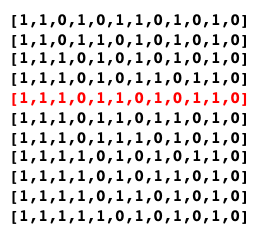
\includegraphics[width=0.4\textwidth]{BeatBox_4}
\end{figure}

%
%[1,1,0,1,0,1,1,0,1,0,1,0]
%[1,1,0,1,1,0,1,0,1,0,1,0]
%[1,1,1,0,1,0,1,0,1,0,1,0]
%[1,1,1,0,1,0,1,1,0,1,1,0]
%[1,1,1,0,1,1,0,1,0,1,1,0]
%[1,1,1,0,1,1,0,1,1,0,1,0]
%[1,1,1,0,1,1,1,0,1,0,1,0]
%[1,1,1,1,0,1,0,1,0,1,1,0]
%[1,1,1,1,0,1,0,1,1,0,1,0]
%[1,1,1,1,0,1,1,0,1,0,1,0]
%[1,1,1,1,1,0,1,0,1,0,1,0]
%

\paragraph{The Exhibit:} 
Go and clap along. Try to start slowly and increase your speed. Select the different shifts by moving the green point on the circle.


\subsection{Sequencer}
Have you ever stepped in to a printing hall of a big newspaper?
Where the machines spin round and round and create a sound pattern with each rotation. Or just listened to a sewing machine? Whenever some mechanical process produces a repeating pattern our brain is trained to search for structure in it. Forming rhythm. Forming music. The beat machine in our exhibition is a sequencer that lets you experiment with cyclic patterns. Play and explore.

\paragraph{The Exhibit:}
Perhaps a little usage description is useful here. Consider the four big wheels as turntables equipped with bars. Whenever the bars hit an instrument it creates a sound. The instruments are resembled by the five small colored points in the central area. You can move them around freely. If they get hit they make a sound. Which instrument is resembled by each point can be chosen by the colored sliders at the far right. The further out an instrument is on a wheel, the louder it is played.

When the machine is at rest, the number of bars on each disk can be changed by moving the sliders. By this, it is possible to create very uneven but still cyclic repetition patterns. For instance you can set one of the disks to 8 bars per turn, the other to 11 and the other two to 15. This sounds wild but still very rhythmic. As a matter of fact, African music cultures are by far more used to such uneven rhythm distributions than Western ones.

\begin{figure}[h]
\centering
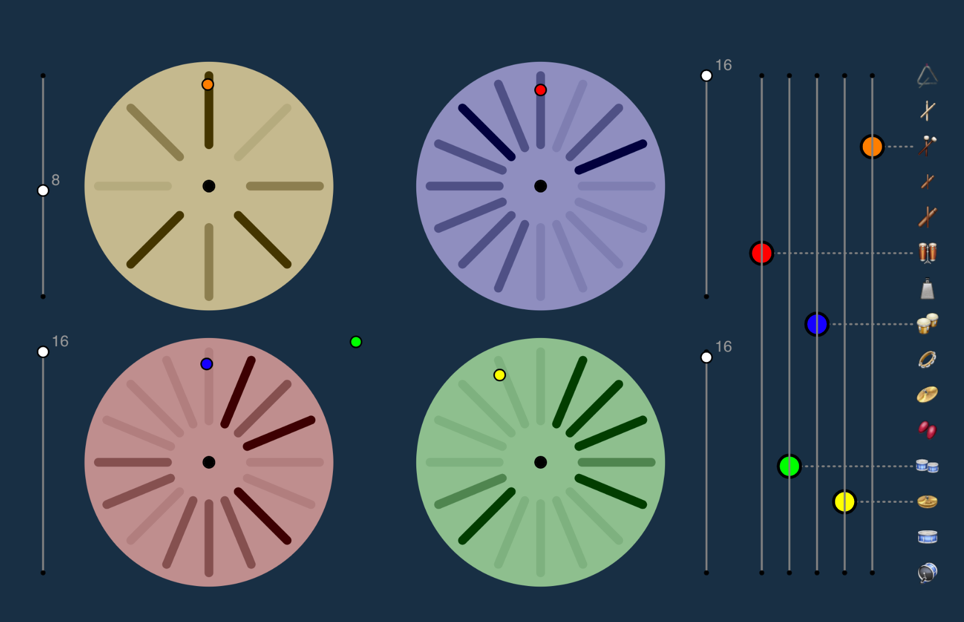
\includegraphics[width=0.9\textwidth]{BeatBox_5}
\end{figure}

In the rest state you can also click on the bars on the disk and alter them between three states, loud-medium-off. By this you can create a great variety of known and of totally new rhythms.


\subsection{n over m Rhythms}
We are very much used to clap simple regular rhythms like a two-step march 1-2-1-2-1-2 or a waltz in a three fold pattern 1-2-3-1-2-3. It is perhaps one of the first exercises when learning a percussion instrument to be able to perform these kinds of rhythms. But things become really difficult if we want to clap two rhythms simultaneously. Combining a regular rhythm with n beats in a bar with another rhythm, that has m beats in the same time is called an n over m rhythm. The speed ratio between the two rhythms is then n/m. The picture below illustrates a 2 over 3 rhythm. In each bar the top voice has exactly two evenly distributed notes while the lower voice has three evenly distributed notes.

\paragraph{The Math:}
Perhaps the easiest way to learn simple n over m rhythms is to merge them into a common framework of constant ticks fine enough to incorporate both rhythms. Mathematically this asks for the least common multiple of the two numbers n and m. Thus a 2 over 3 rhythm can be embedded in a regular rhythm of 6 ticks, a 3 over 4 rhythm can be embedded in 12 ticks and a 7 over 5 rhythm can be embedded into a rhythm with 35 ticks. If one counts the ticks by starting from zero the  m-beat rhythm is played on the multiples of n and the n-beat rhythm is played on the multiples of m.

\begin{figure}[h]
\centering
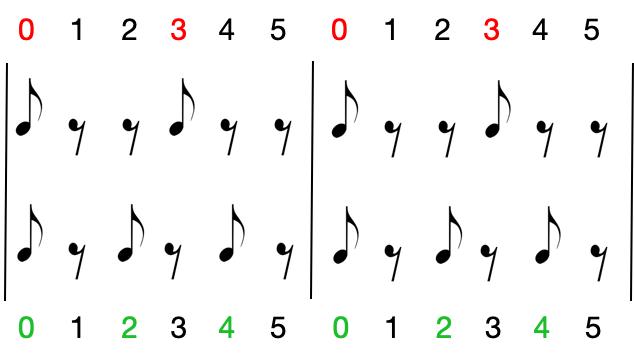
\includegraphics[width=0.7\textwidth]{BeatBox_6}
\end{figure}

\paragraph{The Music:} Playing the n over m rhythm in the above way is a good way to learn it. However it has one big disadvantage. One does not ``feel'' the rhythm as being composed from two distinct regular ones. 

Here is a ``pro tip'' for learning these rhythms. First learn to clap them with two hands by using the above method (it will take a while). After feeling secure in clapping these rhythms play them and ``split your mind'' and focus to only one hand and what it does. And then switch the mind between the two hands. At some point you will be able to feel both rhythms independently and simultaneously in your mind.

\begin{figure}[h]
\centering
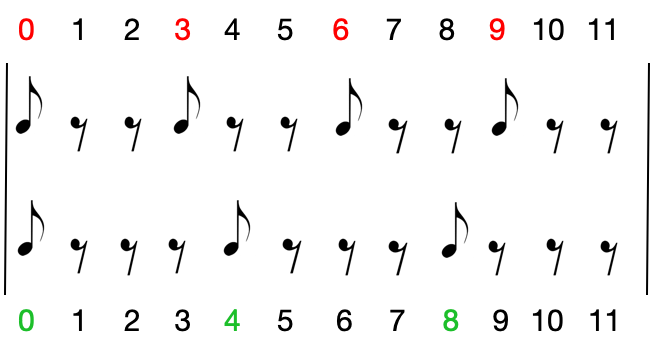
\includegraphics[width=0.7\textwidth]{BeatBox_7}
\end{figure}

\paragraph{The Exhibit:} The exhibit is a clap along exhibit. You can hear and experience n over m rhythms and you can also try to learn clapping them. It might take a little practice but once you get it you won't un-learn.


\subsection{Grid Rhythms}
Can you hear the rhythm of a regular ornamental drawing? Have you ever rushed with a trolley over a regular pavement busy to get your train or airplane? Did you listen to the sound it created? In fact already for the simplest geometric patterns (like a square grid) moving a point over it in constant speed creates interesting rhythmical patterns. If you associate different voices to the horizontal and vertical lines of a grid then moving a point in any direction with constant speed over the grid creates a regular rhythmic pattern in each voice. However the two patterns have different speed and are shifted in phase, leaving lots of space for musical experience.

\paragraph{The Music:} Getting inspirations for interesting musical patterns is an important part of the work of creative musicians. Those inspirations can come from very different sources. 

We strongly recommend to listen to the YouTube Video ``Stoiber on Drums'' in which a percussionist performs along with Edmund Stoibers speech about a fast train connection from Munich Center to the Airport trying to hit an instrument every time there is a syllable in the speech.  

\begin{figure}[h]
\centering
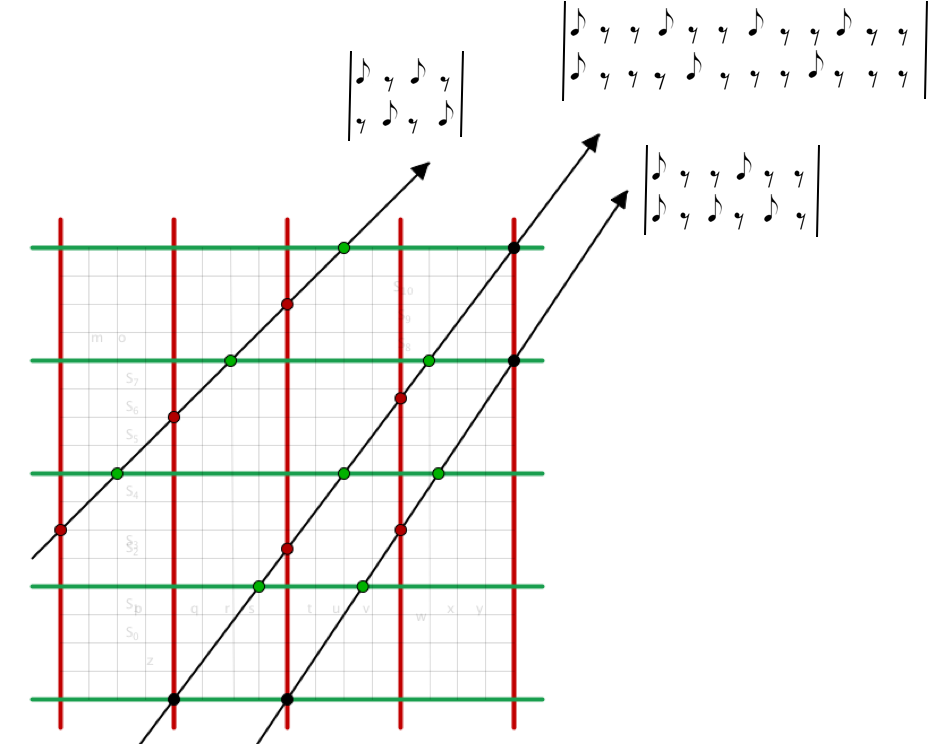
\includegraphics[width=0.7\textwidth]{BeatBox_8}
\end{figure}

\paragraph{The Math:} The square grid creates an overlay of two regular beat patterns. As a matter of fact except for the regularity of each pattern everything else is free in this context: both speeds and the phase between them. The examples in the figure show a few instances, among them a 2 over 3 and a 3 over 4 rhythm. If the slope of the line is irrational (not a fraction) then the rhythmic pattern generated will even never repeat.

\paragraph{The Exhibit:} By adjusting the slope of the movement you can experience all possibilities that are accessible through that approach of rhythm generation. You can adjust the direction of the grid motion. Pressing one of the synchronize buttons sets the grid to the indicated position with respect to the measuring point. This allows you to get a bit more control over the rhythm. 


\subsection{Euclidean Rhythm / Line Step Rhythms}
How to distribute 3 drum hits in a measure of 8 beats? And what does this have to do with low resolution computer screens? Here is a nice connection. Imagine you want to draw a line with slope 3/8 on a low resolution grid by a pixelized line. The picture below indicates the line as a sequence of highlighted pixels. The steps in that image form a regular and rhythmic pattern. The slope of 3/8 implies that while you go 8 units to the right you must go also 3 units up. Thus the pattern repeats after 8 steps. If you hit a drum every time you step up, you get a nice pattern of 3 hits distributed over 8 beats.

\begin{figure}[h]
\centering
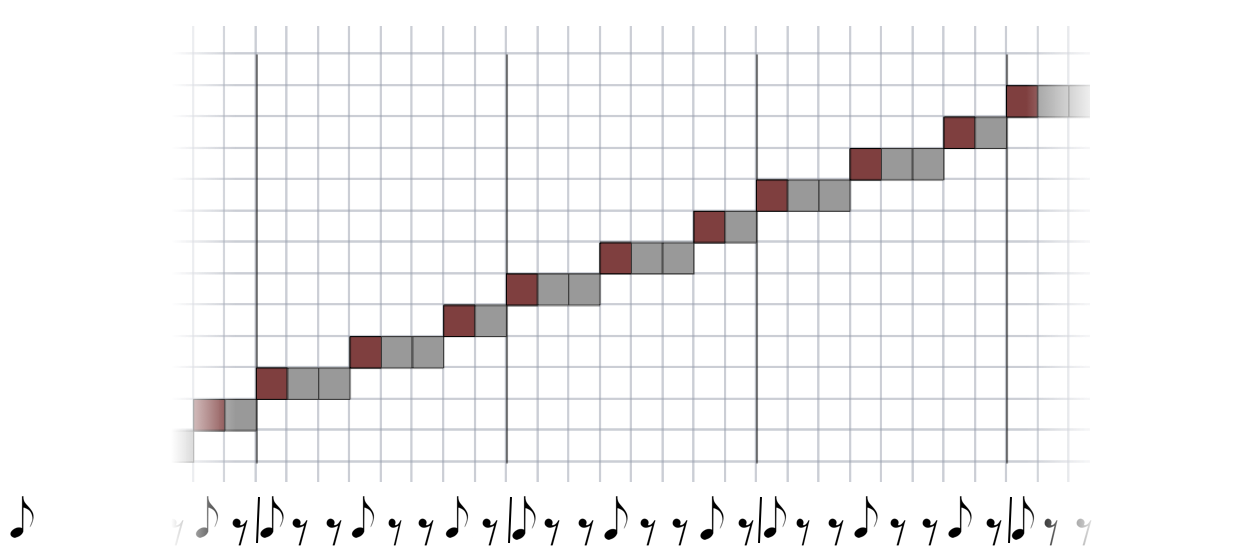
\includegraphics[width=0.7\textwidth]{BeatBox_9}
\end{figure}

\paragraph{The Math:} This generation method for a rhythm has a remarkable property. It distributes the 3 hits as equal as possible among the 8 beats. The reason for that is that the pixelized drawing of the line approximates the line as good as possible. Another way to think about this generation method is to consider an equilateral triangle and then to choose points from an octagon with same centre that are as close as possible to the corners of the triangle. Clearly the method can easily be generalized to any number of hits and beats.

\paragraph{The Music:} The equal distribution indicated by this method creates very interesting rhythms. As a matter of fact they can be found across all different cultures and styles from Balkan folklore, via Latin American and Japanese rhythms, to Dave Brubeck's Take Five and Unsquare dance.

\paragraph{The Exhibit:} In the exhibit you can create two such rhythms in parallel and vary the numbers that generate the rhythms. It is a great device to create and exercise quite complicated and elaborate rhythm patterns.  

\begin{figure}[h]
\centering
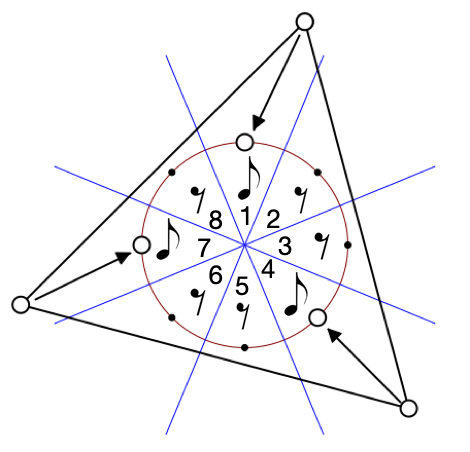
\includegraphics[width=0.4\textwidth]{BeatBox_10}
\end{figure}

\vfill

Author of this exhibit: Jürgen Richter-Gebert, Technical University of Munich 
Sound Engine: Patrick Wilson and Aaron Montag / based on CindyJS.org
Text: Jürgen Richter-Gebert (TU Munich)




\section{Graph Composer}
Un graf és un objecte matemàtic consisteix en un conjunt de vèrtex i arestes que els connecten. També és possible que coneguis els grafs sota el nom de xarxes. Cada vèrtex té diversos atributs o valors en funció del que s'està modelant. Les arestes poden tenir direccions i en aquests casos parlem de grafs dirigits.

El mòdul Graph Composer ofereix la possibilitat de fer música amb el pas per un graf. Cada vèrtex s'associa amb una nota i la seva duració en el temps. Les arestes que connecten els vèrtexs defineixen un camí pel què es pot viatjar a amb el temps. Això signigica que les notes es toquen en l'ordre dels vèrtexs visitats. El so que s'obté de cada vèrtex té diferents formes en funció del decorador del vèrtex, com ara una nota pura, un acord o un arpegi.

Per exemple, la següent partitura:
\begin{figure}[h]
\centering
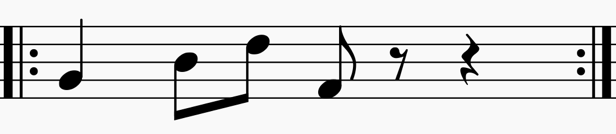
\includegraphics[width=0.5\textwidth]{GraphComposer_1}
\end{figure}

Es pot dibuixar com el següent graf dirigit:

\begin{figure}[h]
\centering
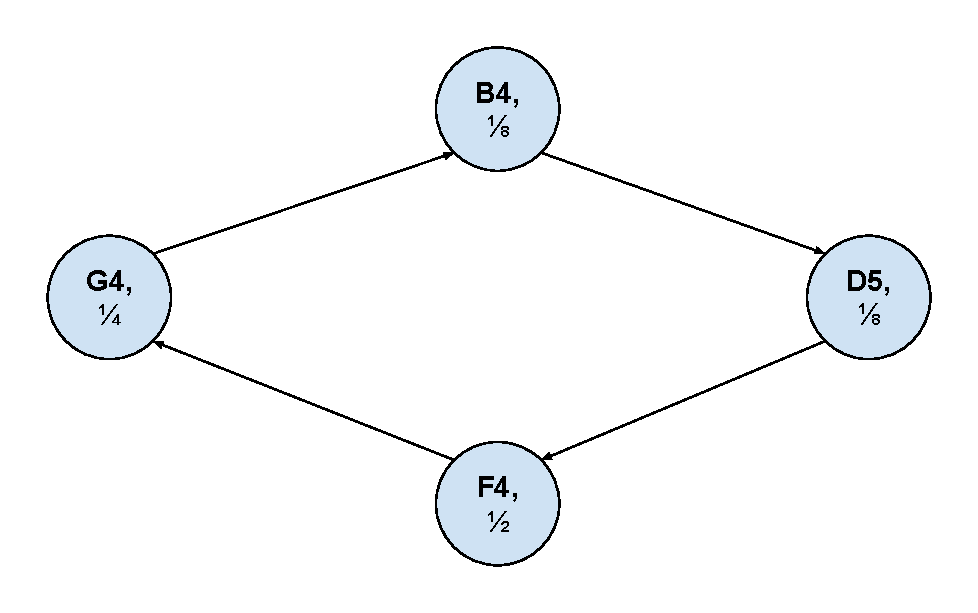
\includegraphics[width=0.5\textwidth]{GraphComposer_2}
\end{figure}

Els camins al graf representen seqüències de notes. Si el camí té un bucle, com a l'exemple d'abans, hi ha la repetició del fragment. A l'exemple, el graf té només un camí possible, però ,quan hi ha més d'una aresta sortint d'un vèrtex, hi ha diversos camins possibles.

Per exemple, el graf que veuràs a continuació té dos possibles camins:

\begin{figure}[h]
\centering
\begin{subfigure}{0.45\textwidth}
\centering
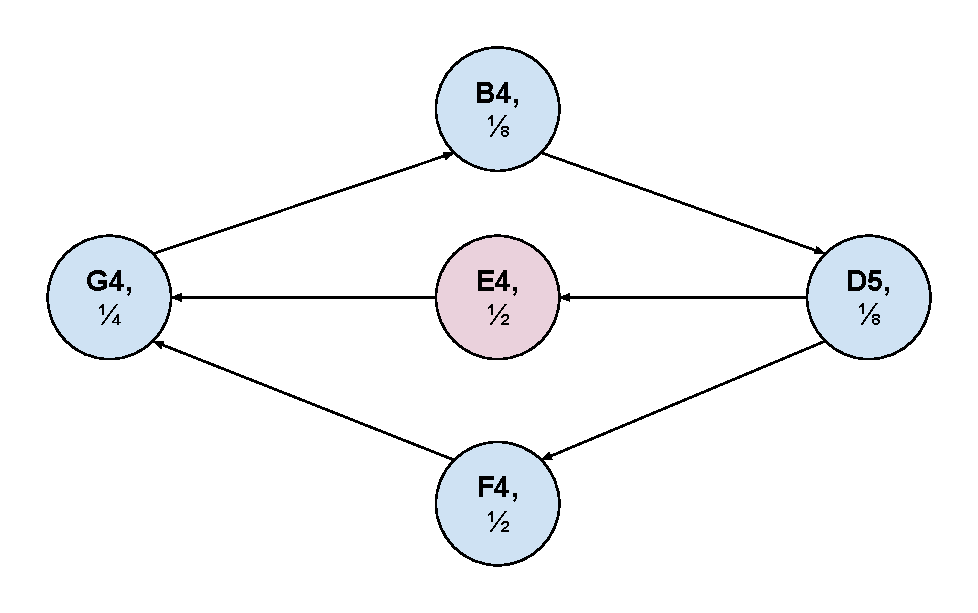
\includegraphics[height=3cm]{GraphComposer_3}
%\subcaption*{This graph can be walked through two paths.}
\end{subfigure}

\begin{subfigure}{0.45\textwidth}
\centering
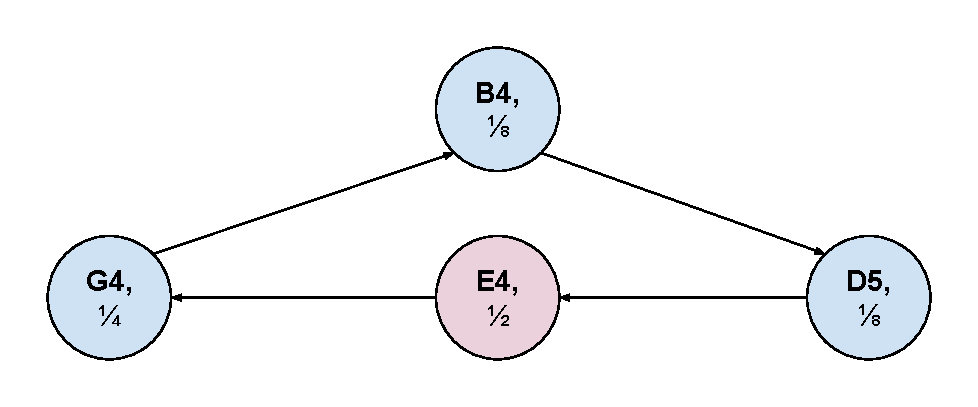
\includegraphics[width=\textwidth]{GraphComposer_5}
%\subcaption*{First path.}
\end{subfigure}
\begin{subfigure}{0.45\textwidth}
\centering
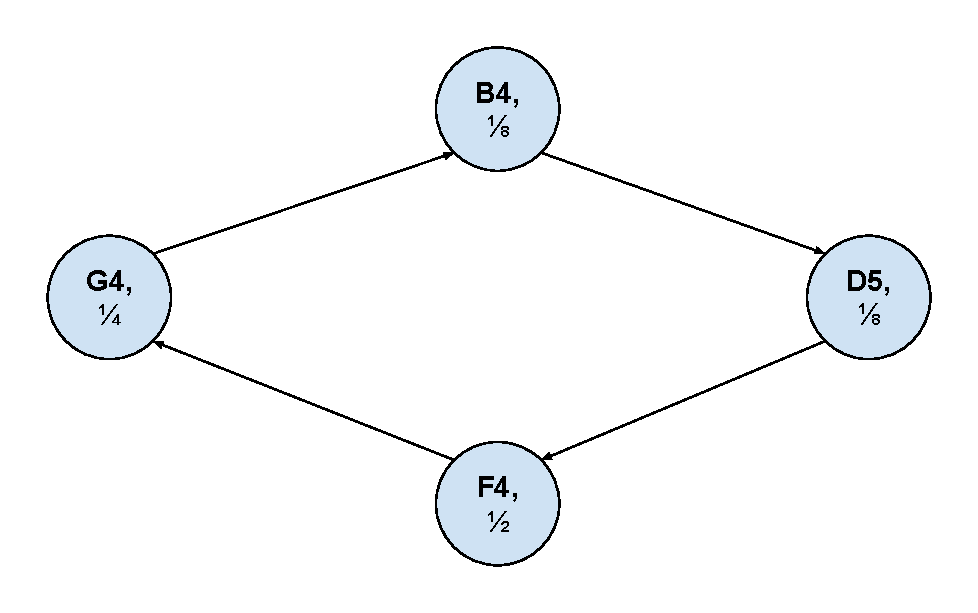
\includegraphics[width=\textwidth]{GraphComposer_4}
%\subcaption*{Second path.}
\end{subfigure}
\end{figure}

En aquest cas, el programa necessita prendre la decisió de quin camí seguir sobre el graf. Aquest mòdul tria de forma aleatoria entre les dues opcions (amb igual probabilitat), i això crea el que s'anomena com a passeigs aleatoris pel graf. Com que la música que produeix cada camí pot resultar en diferents longituds i, per aquest motiu, en una duració diferent de la música. Això pot fer que qui l'escolti la percebi com una mena de ``no-ritme''.

El model utilitzat pel Graph Composer s'utilitza en Musicologia Computacional, un camp d'estudi on les matemàtiques i la informàtica s'apliquen a la música. A la recerca, les composicions musicals es modelen amb grafs per comparar-les i extreure'n diferents propietats matemàtiques. Per exemple, el nombre de vegades que es repeteix la transició d'una nota a una altra, el nombre de vegades que tres o més notes apareixen en el mateix ordre i d'altres.

El Graph Composer passeja pels grafs de forma aleatòria des del vèrtex inicial a través de les arestes dirigides fins que troba un vèrtex amb cap aresta de sortida. Després d'això torna al vèrtex inicial. Quan el programa s'inicia, només pots veure el vèrtex inicial (l'únic que es toca sense cap aresta entrant). Pots arrossegar i afegir més vèrtex, canviar les seves notes, la duració i les decoracions. Tot això es pot fer sense la necessitat de parar la música. La complexitat del graf pot incrementar molt ràpidament a mesura que afegeixes vèrtex. Pots crear patrons al teu graf que creïn motius musicals agradables? Que vagi de gust.

\begin{sectcredits}
\item[Autors del mòdul:] Pedro Arthur, Vitor Guerra Rolla, i José Ezequiel Soto Sánchez (Instituto de Matemática Pura y Aplicada, Brazil).

\item[Text:] Pedro Arthur, Vitor Guerra Rolla, i José Ezequiel Soto Sánchez.

\end{sectcredits}

\section{AI Jam}
Machines can generate and play music, but how good are they at making music together with humans? Could they be part of a Jam Session? Could an Artificial Intelligence eventually replace a missing musician during a band rehearsal?

Even leaving aside questions of musical quality, there are many issues that arise when attempting to compose music using machine learning. One of them, is the generation of a melody. Humans are usually good at producing long-term structures, but machine learning algorithms are not, so the music they produce might sound good on a note-to-note basis, but its structure will seem random and wandering after some bars. AI Jam tackles this problem by explicitly training its Recurrent Neural Network \footnote{\url{www.en.wikipedia.org/wiki/Recurrent_neural_network}} (RNN) with musical structure in mind. When feeding it with thousands of musical pieces, the input was specially labeled whenever a bar was repeating the one immediately preceding it, or the one before that. This is called a Lookback \footnote{\url{www.magenta.tensorflow.org/2016/07/15/lookback-rnn-attention-rnn}} RNN by its developers, the Google Magenta team.

A second technique used is that of Attention. In this case, whenever the RNN produces some output, it looks back at the previous n outputs (with n being configurable), weights them using a calculated attention mask and adds the result. The result is basically the previous n outputs combined, but each given a different amount of emphasis. It is then combined with the output of the current step. In this way, each step produces an output that is related to the previous ones.

By using both mechanisms together, the algorithm can not only produce short fragments of notes that sound good by themselves, but that also form a nice sounding melody when played after a fragment played by a human.

\vfill

Author of the exhibit: Sebastian Uribe (Exhibit conception and project management), Eric Londaits (Software development), Christian Stussak (Additional software development and OS configuration), and Daniel Weiss (Case design and construction) for IMAGINARY.
Original software (based on): Yotam Mann, the Magenta and Creative Lab teams at Google.


\section{Con Espressione!}
A piece of music can be described with mathematical accuracy on a score, with symbols perfectly defined in a well-founded theory. However, music is above all an art, and as such it conveys emotions, feelings, and human sensations. How is it possible to express these feelings, given such a strict notation? How can a performer make a piece come alive? What lies beneath the score sheet and the execution of a piece?
 
A human performer does not play all the notes of a chord at the same time, nor do they keep a strict tempo; some notes start a few milliseconds earlier, or are released a few milliseconds later, some are played louder than others, some appear quicker, etc. All these nuances allow a performing musician to express themselves and imprint some feelings and emotions onto the performance. A musician is not a machine that perfectly reproduces the score, and these ``imperfections'' or deviations are what make the music alive, something that humans do naturally but a machine could never do... or could it?	

This exhibit allows you to explore the difference between a mechanical reproduction of a piece and a more ``human'' interpretation produced by an Artificial Intelligence that was trained to behave as a musician. The visitor takes the role of a music conductor, controlling overall tempo and loudness of a piano performance. Via a camera sensor, the hand of the visitor is tracked in space. The up-down position determines the loudness (volume) of the music, and the left-right position determines the tempo (the speed) of the music. Initially, this is achieved by directly adapting the loudness and tempo of the overall piece according to the position of the hand, but even if the machine obeys you to set these values, the music feels automatic and soul-less. This is because with your hand movements, you can only control overall tempo and loudness, but not the fine details of a performance (such as how to play the individual notes, or how to stress the melody line).

Then, a slider allows you to activate the Artificial Intelligence. The higher the value, the more freedom has the machine to choose small deviations from the prescribed parameters. The machine adjusts the tempo and loudness to be slightly different from what you conduct, to make the music more lively and less ``mechanical''. It also introduces changes in the dynamic spread, micro-timing, and articulation.

\begin{itemize}
\item The loudness is the volume, i.e. the amount of amplification of the sound of each note. Raising the loudness is the most obvious way to stress a note.
 
\item Dynamic spread relates to loudness differences between simultaneously played notes (e.g., in a chord). This is important to make the melody line come out clearly and to change the overall ``sound'' of a chord.

\item Musical tempo is defined as the rate at which musical events or beats are played. Music performers continually change the tempo, speeding up or slowing down, to express the ``ebb and flow'' of the music. This is what makes music sound natural to us (and we may not even be conscious of all these tempo fluctuations).

\item Microtiming refers to the moment that a note plays with respect to its supposed onset. For example, if a chord consists of several notes that are supposed to be played together, one can advance one note over another by a few milliseconds, so that not all of them are perfectly synchronized. This is inevitable in real-life performance, and it makes the piece more warm, human and expressive.

\item Articulation here refers to the duration of a note with respect to its supposed duration according to the score. Notes can be played a bit longer or shorter than the composer described in the score, tying them together or separating them, which helps to stress or diffuse some notes amongst the others. In musical language, this is described with terms as legato and staccato.
\end{itemize}

Each performer has their own experience, understanding of a piece, and expressive intentions, and communicating these in a performance requires control over musical parameters at many levels -- from precise note-level details like articulation or micro-timing to high-level, long-term tempo and the shaping of its dynamics. The computer program behind this exhibit was trained with hundreds of real-life performances of music pieces to analyze and learn how these parameters are used and controlled in real-life interpretations by human pianists. Experimental results show that computers are already very good at learning the low-level, detailed decisions, but still have problems understanding the larger-scale form and dramatic structure of music, and the high-level shaping this requires. Thus, the exhibit explores and demonstrates a compromise: you control overall loudness and tempo with your hand, at a high level, based on your understanding of the music, and the computer adds its own local details and deviations. In this way, the resulting performance is the product of a true cooperation between a human (you) and a computer (AI).

\vfill

Authors of the exhibit: Gerhard Widmer, Florian Henkel, Carlos Eduardo Cancino Chacón, Stefan Balke (Institute of Computational Perception, Johannes Kepler University Linz, Austria
Austrian Research Institute for Artificial Intelligence (OFAI), Vienna, Austria), and Christian Stussak, Eric LONDAITS (IMAGINARY). Text: Daniel Ramos (IMAGINARY).

Acknowledgment: This project has received funding from the European Research Council (ERC) under the European Union's Horizon 2020 research and innovation programme (grant agreement number 670035).

References:

Gerhard Widmer (2017). Getting Closer to the Essence of Music: The Con Espressione Manifesto. ACM Transactions on Intelligent Systems and Technology (TIST) 8 (2), 19. \url{www.arxiv.org/pdf/1611.09733.pdf}

Carlos Eduardo Cancino-Chacón (2018). Computational Modeling of Expressive Music Performance with Linear and Non-linear Basis Function Models. PhD Thesis, Johannes Kepler University Linz (JKU). \url{www.cp.jku.at/research/papers/Cancino_Dissertation_2018.pdf}

Carlos E. Cancino-Chacón, Maarten Grachten, Werner Goebl and Gerhard Widmer (2018). Computational Models of Expressive Music Performance: A Comprehensive and Critical Review. Frontiers in Digital Humanities 5, Oct. 2018. \url{www.frontiersin.org/articles/10.3389/fdigh.2018.00025/full}


\section{NSynth}
Pots mesclar i barrejar sons? Quin és el resultat de barrejar el so d'una guitarra i d'un piano? I el de barrejar el so d'un motor de cotxe amb el d'una flauta?

Un sintetitzador és un dispositiu que genera sons de manera que es pot utilitzar com a instrument. Els sintetitzadors analògics clàssics utilitzen oscil·ladors i filtres, els sintetitzadors digitals moderns funcionen amb mostres emmagatzemades. De tota manera, en tots dos casos, cal descriure el timbre amb precisió mitjançant l'ajustament fi de paràmetres per obtenir el so final que desitgem. Tradicionalment, això es feia manualment amb l'anàlisi del so d'instruments reals (l'espectre i la forma d'ona), o un expert ``esculpia'' la forma d'ona a mà.

Trobar un so ``a mig camí'' entre dos altres sons no és fàcil, ja que els paràmetres són altament no lineals. Si agafes la mitjana de dues formes d'ona (o espectres) de dos instruments, matemàticament això significaria fer-ne la suma, tot el que en trauries seria el so dels dos instruments tocats alhora, no un nou instrument. En comptes d'això, el que realment cal són característiques que defineixen el so dels dos instruments, com ara com de ``brillant'' és, la seva  ``multifonia'' o ``percussivitat''. Llavors, el que realment busques és un sò que sigui la mitjana de ``brillant'' i amb la mitjana de ``multifonia'' o ``percussivitat'' dels dos sons originals.

El NSynth és un sintetitzador que utilitza Intel·ligència Artificial per interpolar i barrejar sons. Una Xarxa Neural Profunda (Deep Neural Network) es va entrenar amb milers de mostres de sons per extreure'n les 16 característiques (dimensions) per cada pas de 32 ms (un total de 2000 paràmetres per les mostres de 4 segons). Amb aquest procés, cada so es codifica amb aquestes dimensions com a paràmetres i, fent el procés a la inversa, aquests paràmetres també ens permetrien crear sons. La correspondència no és perfecta, el so que pots fer amb certs paràmetres no és exactament el mateix que l'original, però sona extremadament proper i molt similar. I, el que és més important, ara pots barrejar aquests paràmetres de forma lineal els uns amb els altres per generar nous sons que tinguin realment la mitjana de les qualitats dels sons originals.

El dispositiu NSynth de l'exposició conté la Xarxa Neural entrenada i pot interpolar quatre sons seleccionats (utilitzant les quatre rodetes que incorpora). Tocant un punt al sensor tàctil quadrat, el sintetitzador ajusta els paràmetres per fer-los proporcionals a les coordenades del quadrat.  Els quatre sons originals s'associen a les cantonades, tota la resta de punts corresponen a sons nous.

\begin{figure}[h]
\centering \small
\begin{tikzpicture}
\node at (0,0) { 
\includegraphics[width=0.7\textwidth]{NSynth_1_nolabels} };
%\draw[step=1,gray,very thin] (-3,-3) grid (3,3);
\node at (0.6,2.6) [align=center, anchor=south]
    {Pantalla};
\node at (-2.5,-0.4) [align=center, anchor=east]
    {Selectors \\ d'instruments};
\node at (2.9,-0.2) [align=center, anchor=west]
    {Interfície \\ tàctil};
\node at (0.5,-2.2) [align=center, anchor=north]
    {Controls d'envolvent};
\end{tikzpicture}
\vspace{-2em}
\end{figure}

\paragraph{Selectors d'instruments} - Aquests instruments s'assignen a les cantonades de la interfície tàctil.

\paragraph{Pantalla} - Mostra l'estat de l'instrument i altra informació addicional sobre els controls amb què estàs interactuant.

\paragraph{Controls d'envolvent} - S'utilitzen per personalitzar encara més la sortida que genera el dispositiu.
\begin{itemize}
\item ``Posició'' fixa la posició inicial de l'ona. (Talla l'atac de la forma d'ona o comença des de la cua).
\item ``Atac'' controla el temps que triga la pujada inicial des de zero fins al pic.
\item ``Caiguda'' controla el temps que triga la baixada des del pic de l'atac fins al nivell que es desitja mantenir.
\item ``Sustent'' ajusta el nivell que tindrà la seqüència principal del so fins que la tecla es deixi anar.
\item ``Alliberament'' controla el temps que triga el nivell fins a tornar a 0 després que es deixi anar la tecla.
\item ``Volum''  ajusta el volum general de la sortida del dispositiu.
\end{itemize}

\paragraph{Interfície tàctil} - És un sensor capacitiu, com el panell tàctic que simula el ratolí en un ordinador portàtil, i s'utilitza per explorar el món de nous sons que el NSynth ha generat entre els sons font que has seleccionat.

\begin{sectcredits}

\item[Autor del mòdul:] NSynth és un sintetitzador de codi obert basat en Machine Learning desenvolupat pel projecte Googe Magenta. NSynth Super és una interfície de hardware obert desenvolupada pel Google Creative Lab.

\item[Text:] Daniel Ramos (IMAGINARY).

\item[Referències:] \strut
\noindent \begin{itemize}[leftmargin=*]

\item \emph{NSynth: Neural Audio Synthesis}. Website at Google's magenta project. \\
\url{www.magenta.tensorflow.org/nsynth}.

\item Jesse Engel, Cinjon Resnick, Adam Roberts, Sander Dieleman, Douglas Eck, Karen Simonyan, and Mohammad Norouzi. \emph{Neural Audio Synthesis of Musical Notes with WaveNet Autoencoders.} \\
\url{www.arxiv.org/abs/1704.01279}, (2017).

\item \emph{NSynth Super: An experimental physical interface for the NSynth algorithm.} Website at Google's Creative Lab.\\ \url{www.nsynthsuper.withgoogle.com}.
\end{itemize}
\end{sectcredits}

\section{Lissajous-based exhibits}

Les figures Lissajous (que reben el nom del matemàtic francès Jules Antoine Lissajous) són corbes determinades per la intersecció de dos moviments oscil·lants perpendiculars. Matemàticament, les seves coordenades $x,y$ al pla són definides per cada instant de temps $t$ a les fórmules:
$$\left\{ \begin{array}{rcl}
x &=& \sin(a\cdot t) \\
y &=& \sin(b\cdot t + \varphi)
\end{array} \right. $$
on $t$ és el paràmetre del temps (angle), $a$ i $b$ són les dues freqüències, i $\varphi$ és el desfasament entre una i altra. Per diferents valors de temps $t$, les equacions formen una corba dins un quadrat. La seva forma exacta depèn bàsicament de la ràtio numèrica de les dues freqüències. Si $a=b$, o $a/b=1$, llavors la figura es tanca després d'un període i el resultat és una línia o una el·lipse. Si $a/b = 3/2$, la corba tanca després de $3\cdot 2=6$ cicles i és força neta. En general, ràtios de nombres petits resulten en corbes simples. Altrament, si els nombres	tenen ràtios més complexes, com ara $a/b = 23/22$, la corba es tanca després de molts cicles (concretament $22\cdot 23=506$ cicles) i la figura resultant és més densa i desordenada. Per això, les figures de Lissajous són una eina per visualitzar quan dos nombres tenen una ràtio simple.

En aquest cas, les nostres oscil·lacions són el so, i la freqüència del so es percep com el to. A la música, una idea fonamental que es remunta fins a Pitàgores, és que els sons amb freqüències amb ràtios més petites sonen consonants, i freqüències amb ràtios més complicades són menys consonants. Per aquest motiu les figures de Lissajous s'utilitzen per visualitzar consonància o dissonància. Els intervals consonants clàssics són l'octava (ràtio 2:1), la quinta (ràtio 3:2) i la tercera major (ràtio 5:4).

També és possible tenir corbes de Lissajous tridimensionals, anàlogues a les de dues dimensions, però amb tres vibracions perpendiculars en comptes de dues. Tres notes sonant alhora formant un acord de triada, que són la base per la composició musical. En afinació d'entonació justa, els acords majors els formen notes amb ràtios 4:5:6 i els acords menors notes amb ràtios 10:12:15.

És especialment remarcable que aquestes relacions ens produeixen sentiments d'``alegria'' amb els acords majors i ``tristesa'' amb els menors. Jugar amb aquestes relacions es transforma en una aventura per a la composició d'una peça que aconsegueixi transportar emocions.


\section{Galeria de Lissajous}
Les sis figures d'aquest apartat són representacions artístiques de figures de Lissajous. Per crear-les, l'artista Ryan Cashman va començar amb una corba a l'espai definida per dues ones sinusoidals. Això és una figura de Lissajous, però també està modulada per una segona oscil·lació. Amb la ràtio de freqüència escollida, la corba es mou al voltant de si mateixa passant molt a prop però no exactament sobre si mateixa. El programa calcula punts a intervals regulars durant la corba, creant vèrtexs. Els vèrtexs es connecten en ordre per crear la corba base de la forma. Després es dibuixen línies entre qualsevol parell de vèrtexs que estiguin prou a prop a l'espai per crear una representació de la superfície que recorda a una teranyina. Les freqüències escollides per cada imatge són acords en afinació de temperament igual.


Matemàticament, la posició $x$ (eix horitzontal) i la $y$ (eix vertical) de cada vèrtex es calcula amb la fórmula:
$$\left\{ \begin{array}{rcl}
x &=& \sin(f_X\cdot t + \varphi) \cdot \cos(m_X \cdot t) \\
y &=& \sin(f_Y\cdot t + \varphi) \cdot \cos(m_Y \cdot t)
\end{array} \right. $$
on també hi ha, de forma addicional, $m_X$ i $m_Y$ que en són els coeficients de modulació.

\begin{figure}[!h]
\centering
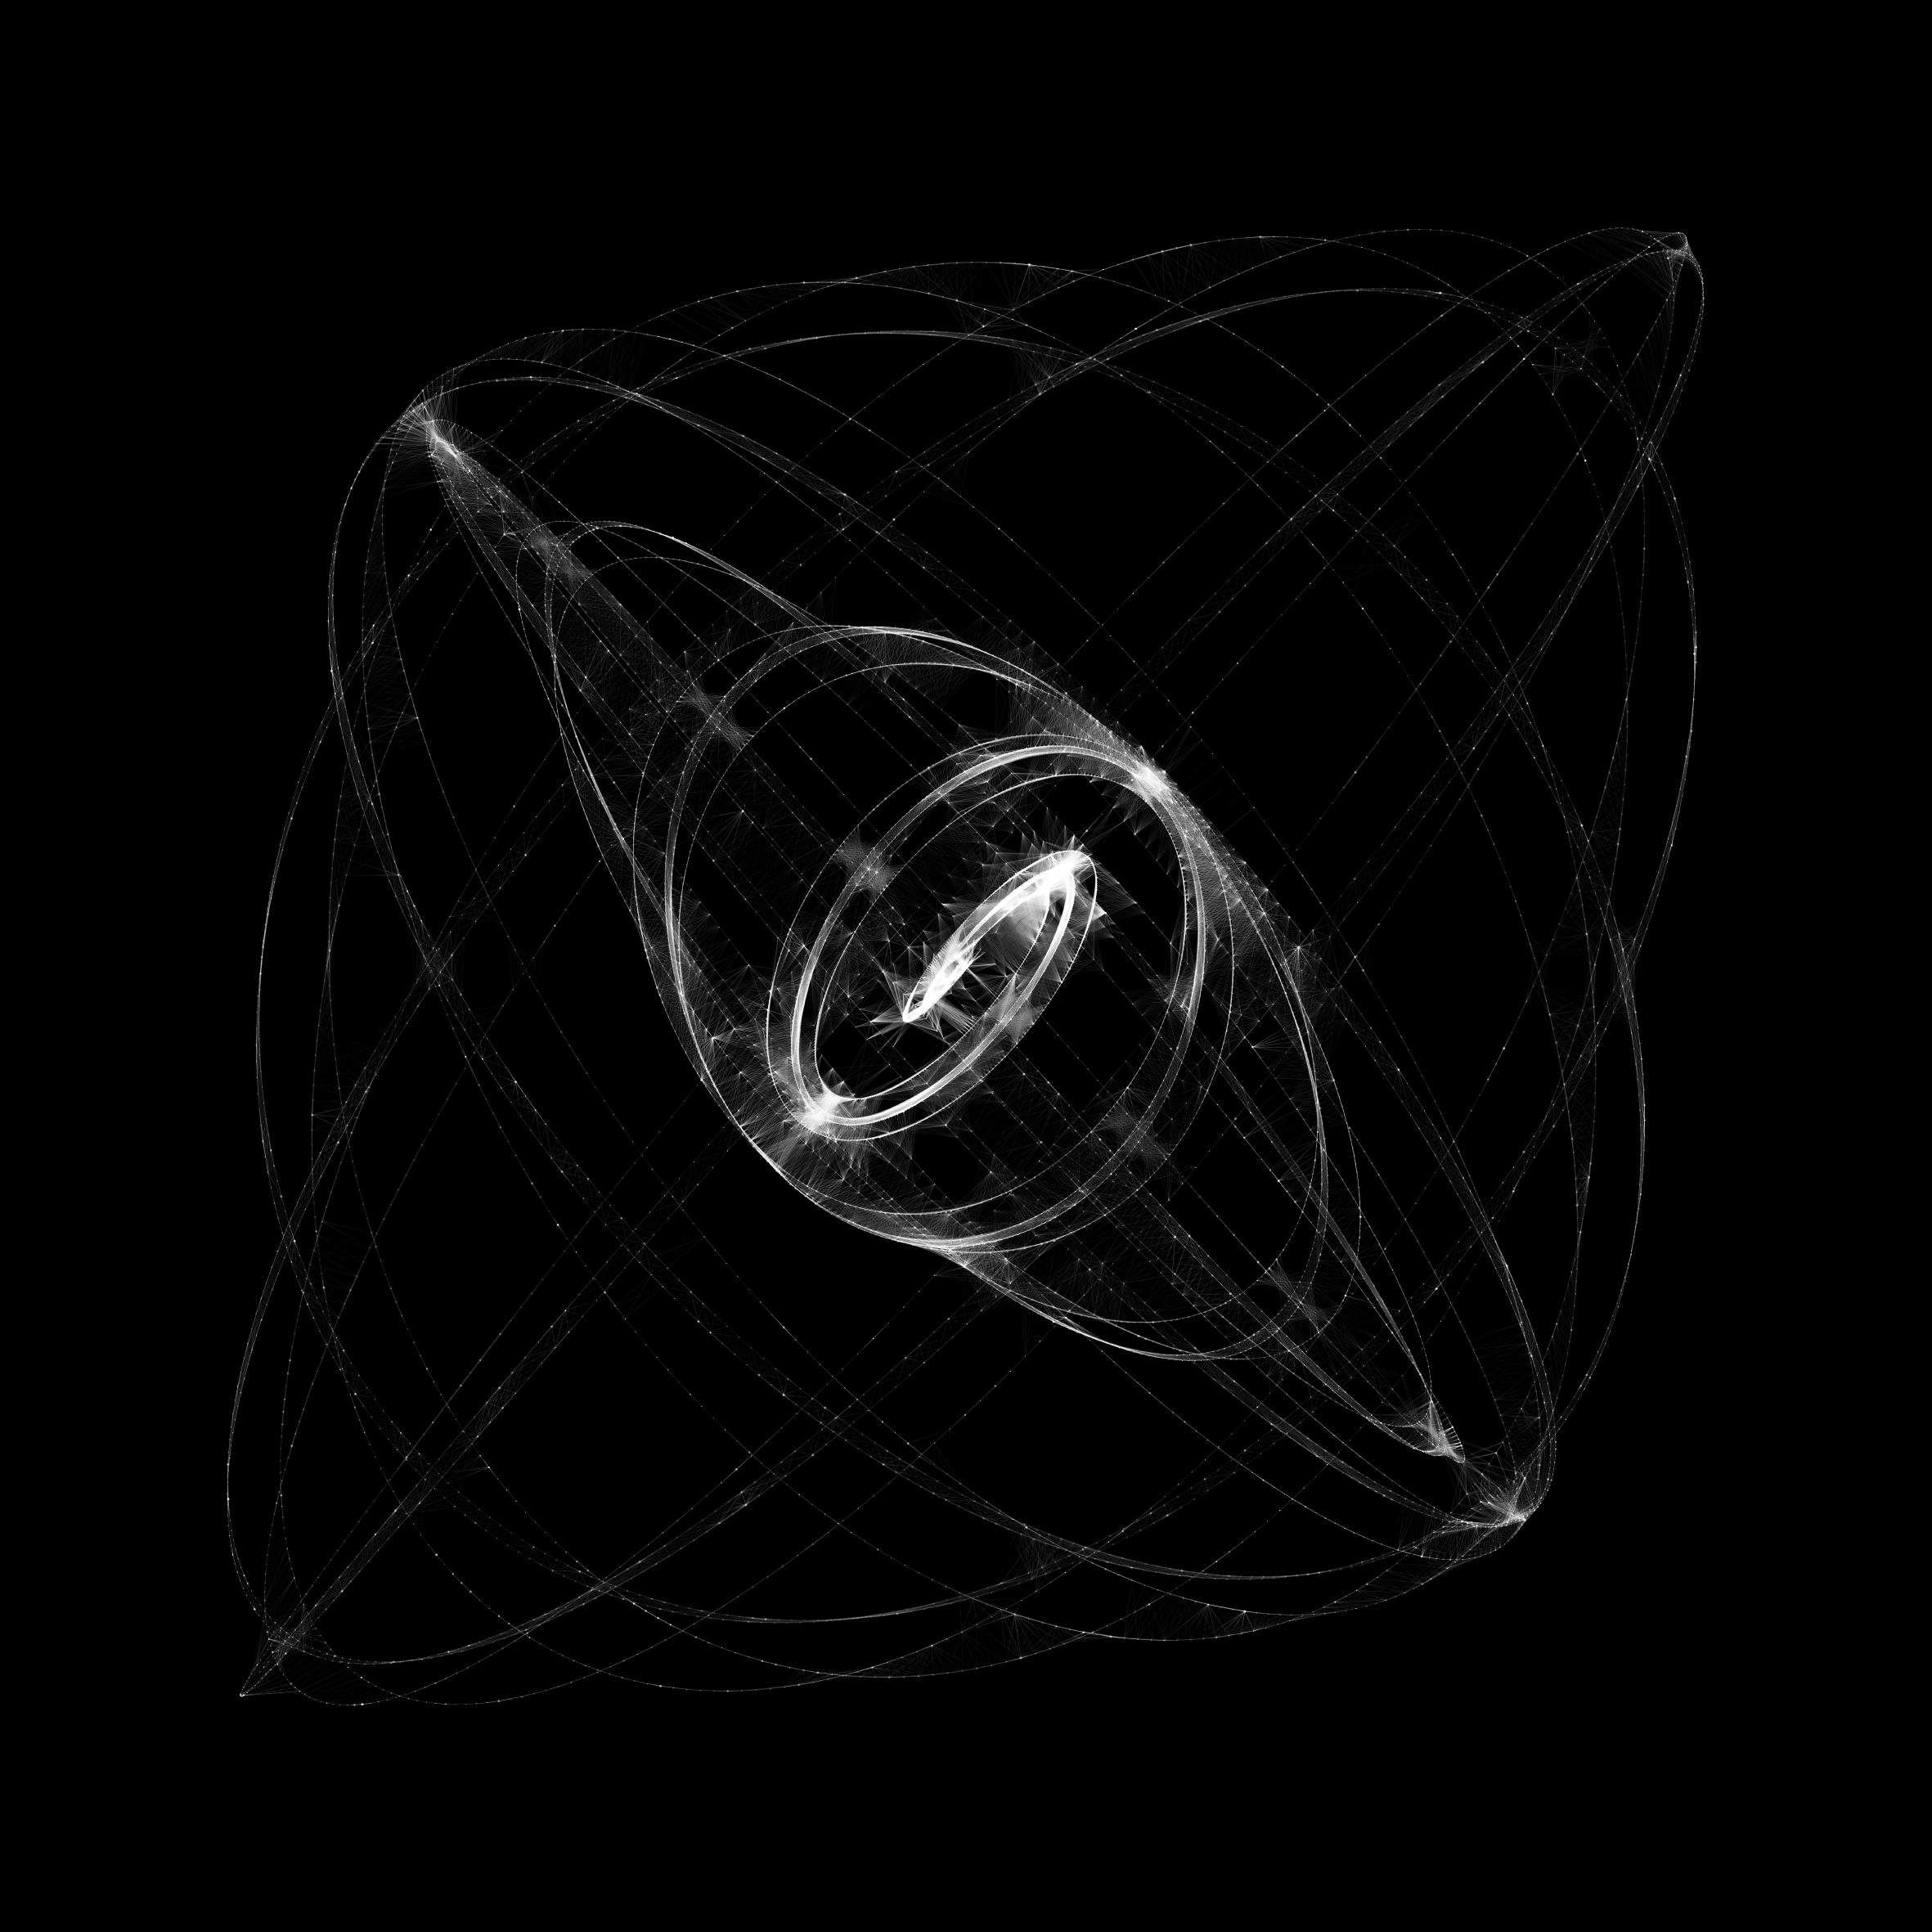
\includegraphics[width=0.6\textwidth]{Lissajous_Cashman}
\caption*{Segona major}
\end{figure}


\begin{sectcredits}
\item[Autor de la galeria:] Ryan Cashman.
\item[Text:] Ryan Cashman.
\end{sectcredits}

\section{Les Sèries Harmòniques}
Quan el Jules Antoine Lissajous va inventar el dispositiu que produeix les corbes amb el seu nom, va ser amb el propòsit d'estandarditzar els sons musicals. Al seu disseny original, dos diapasons es col·locaven de forma perpendicular, cadascun amb un mirall enganxat a un extrem. Llavors es feia incidir un feix de llum sobre el primer mirall, es reflectia cap al segon mirall i finalment a la pantalla. Si les freqüències dels diapasons tenien ràtios simples, cosa que els feia harmoniosos musicalment, les figures dibuixades amb la llum també ho eren visualment.

\begin{figure}[!h]
\centering
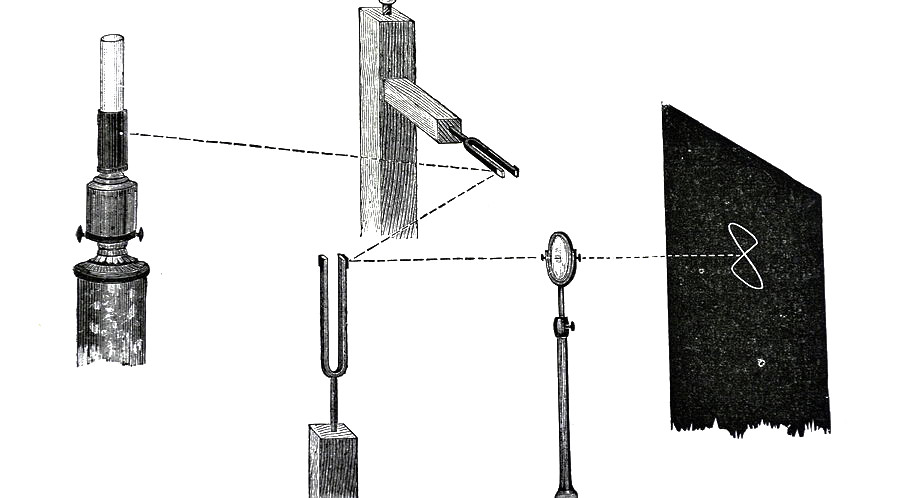
\includegraphics[width=0.6\textwidth]{Lissajous_apparatus}
\end{figure}

Les peces an aquestes sèries que van fer la Manuela Donoso i la Luisa Pereira recreen i estenen el dispositiu de Lissajous utilitzant tecnologia contemporània, portant-ho des del camp de la funcionalitat fins al de l'art interactiva. Els seus dispositius ens conviden a utilitzar les nostres veus per interactuar amb vibracions sonores de forma visual per desenvolupar un enteniment més profund i intuïtiu de la interacció entre soroll, consonància, dissonància i harmonia.



\subsection{Dispositiu \#1}
Micròfons, amplificadors, altaveus, miralls i làser.

Aquest dispositiu afegeix interactivitat a l'aparell original de Lissajous canviant els diapasons per altaveus i la font de llum per un punter làser. Cada altaveu es connecta a un micròfon i els dos miralls col·locats a les seves membranes vibren en direccions perpendiculars. Mentre els altaveus vibren amb les veus dels visitants, les figures projectades evolucionen: els sons percussius generen figures caòtiques, els intervals dissonants generen figures desordenades i els intervals consonants generen figures harmonioses. Si es xiula, les figures resultants són més agudes que si es canten les mateixes notes, fent visible la varietat i la riquesa del timbre a la música.

\subsection{Dispositiu \#2}
Micròfon, amplificador, convertidor analògic-digital, microcontrolador, sintetitzador i pantalla hologràfica.

Aquest dispositiu afegeix una tercera dimensió a les figures de Lissajous, permetent la visualització dels acords de triada. Les dues primeres notes les generen oscil·ladors i els visitants poden ajustar-ne la freqüència movent botons lliscants amunt o avall. La tercera vibració és la que els visitants triïn fer amb un micròfon: poden cantar diferents tons, parlar, xiuxiuejar o experimentar amb qualsevol so que els agradi. Aquest software personalitzat mostra aquestes tres vibracions en un espai tridimensional amb el temps: el primer sintetitzador determina la x, la veu la y i el segon sintetitzador la z de cada punt de la figura 3D resultant. Finalment, la figura es codifica per poder-la mostrar en una pantalla hologràfica, creant una estructura de llum que evoluciona constantment.

\subsection{Escultures de Triada}
Impressions 3D amb estereolitografia.

Les figures tridimensionals de Lissajous representen tres triades diferents: majors (amb ràtios de freqüència $4:5:6$), menors ($10:12:15$), i disminuïdes (aproximadament $20:24:29$). Observa que tant en el cas de les majors i menors, quan agafem parelles de freqüències aquestes tenen ràtios $4:5$, $5:6$, i $2:3$, però les figures de Lissajous (i els acords) no són el mateix. Pots utilitzar un focus per crear una ombra. El nombre de lòbuls a cada costat de la figura plana de Lissajous et dóna  les ràtios.

Aquestes figures es poden reproduir fent que el Dispositiu \#2 rebi tons amb aquestes ràtios, cantant i desplaçant els botons dels sintetitzadors.

\begin{sectcredits}

\item[Autors de les sèries:] Manuela Donoso i Luisa Pereira.\\
Producció (Dispositiu \#1): Manuela Donoso i Lukas Reck per IMAGINARY.\\
Programació (Dispositiu \#2): Luisa Pereira i Ricardo Dodds.

\item[Patrocinat:] Pantalla hologràfica 3D de The Looking Glass (\url{https://lookingglassfactory.com}).

\item[Text:] Manuela Donoso i Luisa Pereira.

\item[References:] \strut \\
\url{www.theharmonicseries.net}

\end{sectcredits}

\section{Pink Trombone}
Voice is the oldest and most complex musical instrument. The human voice organs are unique amongst all the animals and allow us to communicate and express ideas and feelings through sophisticated sounds that we can create and control instinctively.

As an instrument, voice is extremely rich and complex. Some sound characteristics are fixed and particular of each individual, while others can be changed to produce sounds that we can recognize as letters and words. Singing requires the sound to be not only recognizable, but exactly the one intended for the particular piece of music, which demands much more practice and skill. The film station shows a video of the cross section of a singer taken with an MRI (magnetic resonance imaging) machine while singing.

Here we present an interactive simplified model that allows to replicate with certain fidelity the human voice. This model consist of two components: sound production and sound articulation.

The sound is produced in the glottis (throat). This organ has some membranes or vocal folds that we can make vibrate and produce sound when we expel air. With the tension we put on this muscle (vocal cords) and the pressure of the air we expel we can control the pitch of the sound and also the intensity, from a whisper to a shout. Using these parameters the model generates an initial wave form.

The sound wave coming from the glottis enters the vocal tract, where we articulate the sound. Articulation is to modify the voice sound to make a particular speech sound (or phone), that is, the sounds of letters that we use to speak. We can think of a simplified vocal tract as a tube, where the sound wave travels at certain speed (the speed of sound) only in one dimension (forward or backwards). If the tube were completely smooth and uniform, the wave would travel forward uninterrupted until the lips. However, the tube is not smooth nor uniform, and the sound wave bounces back and forth. The main characteristic of the tract is the diameter of the cross section at each point, that we can change with the position of the tongue and lips. Changes in the diameter of the tube make the wave bounce. In this model, the voice tract is a tube of 17 cm divided into 44 sections, each one with a constant diameter.

\begin{figure}[h]
\centering

\includegraphics[width=0.4\textwidth]{PinkTrombone_4}
\end{figure}

The difficulty of propagating a wave through a tube is measured by its impedance $Z$, which is inversely proportional to its area. When the wave passes from a section tube of impedance $Z_i$ to one of $Z_{i+1}$, the reflection coefficient is
$$r=\frac{Z_i - Z_{i+1}}{Z_i + Z_{i+1}}$$
and a fraction $r$ of the wave intensity is reflected backwards, and $(1-r)$ is transmitted forward. The model keeps track of two waves, one moving forward and another moving backwards. By computing the wave intensity (air pressure) at each section at each time step (the time-step is the time required to travel one section of the tube at the speed of sound), we can work out the pressure wave coming from the `lips', which is the sound we hear. The model is improved by including a second tube (the nose), that attaches to the main tube (mouth) at the palatal velum.

On the screen, the voicebox control allows you to choose the pitch (horizontally) and loudness (vertically) of the sound produced at the glottis. 

Clicking on the tongue control, oral cavity, and nasal cavity allows you to modify the vocal tract. The crossing lines represent the diameter of the tract at each section.

\begin{sectcredits}

\item[Author of the exhibit:] Neil Thapen (Institute of Mathematics / Academy of Sciences of the Czech Republic). Adaptations by Eric Londaits (IMAGINARY). 

\item[Text:] Daniel Ramos (IMAGINARY).

\item[References:] \strut 

\noindent \begin{itemize}[leftmargin=*]
\item Julius O. Smith III, \emph{Physical audio signal processing for virtual musical instruments and audio effects}. \\\url{www.ccrma.stanford.edu/~jos/pasp/}

\item Story, Brad H. \emph{A parametric model of the vocal tract area function for vowel and consonant simulation}. The Journal of the Acoustical Society of America 117.5 (2005): 3231-3254.

\item Lu, Hui-Ling, and J. O. Smith. \emph{Glottal source modeling for singing voice synthesis}. Proceedings of the 2000 International Computer Music Conference. 2000.

\item Mullen, Jack. \emph{Physical modelling of the vocal tract with the 2D digital waveguide mesh}. PhD thesis, University of York, 2006.

\item John Coleman. \emph{Acoustics of Tube Models (2): Kelly and Lochbaum method}. \\
\url{www.phon.ox.ac.uk/jcoleman/kelly-lochbaum.htm}

\item Bernard Richter, Matthias Echternach, Louisa Traser, Michael Burdumy, Claudia Spahn. \emph{The voice: Insights into the Physiology of Singing and Speaking}. DVD-ROM, Helbling eds. 2017.

\item Pink trombone (original version): \url{www.dood.al/pinktrombone}
\end{itemize}

\end{sectcredits}


\section{Mind and Music Jukebox}
What are mathematicians and computer scientists favorite songs? What music inspires scientists? What music relaxes them? What music makes them dance?

The Mind and Music Jukebox presents the music of mathematics, or to be more precise, the music of mathematicians and other great minds! We asked mathematicians and researchers from the Women of Mathematics throughout Europe exhibition project and the recipients of the most prestigious awards in mathematics and computer science, namely the Abel Prize, the ACM A.M. Turing Award, the ACM Prize in Computing, the Fields Medal and the Nevanlinna Prize, to fill the jukebox with their beloved music pieces.

What music is your favorite? What music should be the background track of a mathematics class? What music makes you think?

\begin{sectcredits}
\item[Idea and Implementation:] Andreas Daniel Matt and Bianca Violet for IMAGINARY.

\item[References:]
Pictures for this exhibit are from the book \emph{Masters of Abstraction} photographed by Peter Badge, and from the exhibition \emph{Women in Mathematics throughout Europe}, photographed by Noel Tovia Matoff.
\\ \url{www.heidelberg-laureate-forum.org/masters-of-abstraction}
\\ \url{www.womeninmath.net}

\end{sectcredits}

\section{Whitney Music Box}
This mesmerizing applet is inspired by the animations of John Whitney (1917-1995), a filmmaker that explored and experimented with animation techniques governed by mathematical and mechanical rules, before the digital era. In the 1950s, Whitney experimented with pendulums, gears, mechanical artifacts, and early analog computers combined with cameras to produce short films of lines and dots of light, being a pioneer of video as a plastic form of abstract art. In the 1960s he embraced digital computers and devoted his career to computer graphics art, with shorts and films as Permutations (1968), Arabesque (1976), or Moon Drum (1991).

In 1980, Whitney published the book Digital Harmony, where he describes his experiments on visualizing music with computer graphics. In particular, he explains what he called ``incremental drift'', a kind of algorithm to set the position of particles, where each particle is ``drifted'' from the previous one by a simple rule; a kind of differential rule that by integration gives rise to a global behavior that was originally unexpected. Whitney gave in his book an example of this spiral incremental drift. 

In 2006, the programmer and Disney animator Jim Bumgardner took Whitney's ideas and created an interactive applet adding synchronized sound to Whitney's spirals. Bumgardner coined the term ``Whitney's music box'' and the applet has become popular on the Internet since.

\begin{figure}[h]
\centering
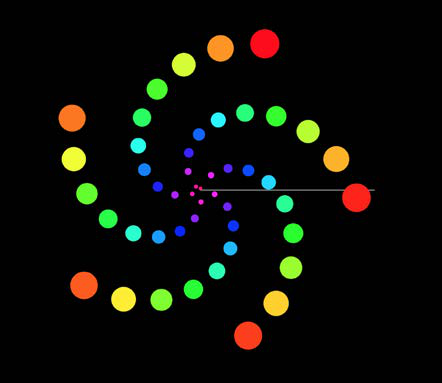
\includegraphics[width=0.5\textwidth]{Whitney_1}
\end{figure}

Mathematically the applet can be described fairly easily. Each point moves along a concentric circle, and moves at an angular speed proportional to its radius. Or said in other words: every time the innermost dot goes once around the circle, the next one goes twice, the next one goes three times, and so forth. 

The overall reference for rotation speed is given by the controlling wheel/knob. Each point plays a particular tone (assigned in the chromatic scale) when the point crosses the horizontal line. This rotations produce changing spiral patterns and chords when several tones play at once. The speed of rotation imposes a rhythmic cadence of tones that reflect the geometry of the pattern, evoking the consonance and dissonance of the notes in the scale.

This music box enables to visualize harmonic resonance and musical harmony in a pleasant way. Playful and challenging in the same time, you might find it hard to predict what will the sound and patterns resemble. It is a tool for admiration and a bit of self-hypnotic recreation.



\vfill

Author of the exhibit: Eric Londaits (IMAGINARY). 
Inspired by Jürgen Richter-Gebert's implementation.
Text: Eric Londaits and Daniel Ramos (IMAGINARY).

References:

\url{https://krazydad.com/blog/2006/04/23/visual-harmony}

\url{https://boingboing.net/2016/04/11/john-whitney-music-box-a-psyc.html}

\url{https://jbum.com/papers/whitney_paper.pdf}

John Whitney. Digital Harmony: On the Complementarity of Music and Visual Art. Byte Books / McGraw-Hill (1980). \url{https://archive.org/details/DigitalHarmony_201611}


\section{Musical Bench}
El mòdul Musical Bench és un mòdul que fa música quan la gent es toca, s'agafa la mà o es fa un petó. Fa servir un microcontrolador per detectar canvis de resistència, via els braços recolzadors, i toca notes més agudes o més greus depenent del corrent que passi per cada parella de visitants. 

Un simple divisor de tensió s'utilitza com a entrada. Com més fort premi una persona o més superfície tingui en contacte amb els panells o fins i tot a més humitat tingui a les mans, menor serà la resistència. Les resistències baixes estan associades a freqüències altes, per això, com més s'arrepengi una persona, més alta serà la nota. Per altra banda, un petit toc provoca notes greus. Amb aquesta informació el xip arpegia l'escala cromàtica. 


\vfill
Construït per: Tobias Hermann per a IMAGINARY.
Basat en la idea de: Exploratorium / San Francisco.

Referències:
Dóna una ullada a aquest web amb les instruccions per fer el teu propi Musical Bench: \url{https://www.exploratorium.edu/tinkering/projects/musical-bench}.
\section{Hands-on Table}
En aquest mòdul trobaràs una taula que et convidarà a començar a explorar i potinejar. Si vols continuar a casa o a l'escola, pots consultar la pàgina web de l'Exploratorium / San Francisco per trobar més instruccions i recursos: \url{https://www.exploratorium.edu/snacks}. Els aperitius científics són activitats ben provades i organitzades que utilitzen materials barats i que pots trobar fàcilment i que cobreixen un ampli ventall de temes. Òbviament, et recomanem que en busquis de ``música'' i ``mates''.

\vfill

Experiments de: Exploratorium / San Francisco
Selecció d'activitats: IMAGINARY.

\section{La La Cinema}

The film station is a collection of short videos focusing on the relation between music and mathematics. The program includes films, videos and animations that have been created for educational, corporate and artistic purposes, or just for fun. The total length of all films is about one hour (1:05 h). We thank all the authors for giving us permission to screen their films within the La La Lab exhibition.

The following films are shown:

\subsubsection*{Peace for Triple Piano (4:15)}
Vi Hart in collaboration with Henry Segerman, with additional help from Sabetta Matsumoto. \\
This is a spherical video in a mathematically triplified space with symmetry in space-time.

\subsubsection*{Making of Peace for Triple Piano (9:42)}
Vi Hart in collaboration with Henry Segerman, with additional help from Sabetta Matsumoto.\\
This video explains the concepts, as well as the math, movie, and piano magic used to create the previous film (Peace for Triple Piano).

\subsubsection*{J.S. Bach - Crab Canon on a Möbius Strip (3:07)}
Jos Leys - www.josleys.com \\
The manuscript depicts a single musical sequence that is to be played front to back and back to front.

La La Relation: Compare this video with the Bach canon in the exhibit `Show me Music'.

\subsubsection*{Improvising a canon at the fifth above (4:22)}
Singers: Peter Schubert, Schulich School of Music, McGill University, Montreal, and Dawn Bailey\\
Production: Tuscan Bean Soup, Montreal\\
Producer: George Massenburg\\
Editor: Michelle Hugill\\
Concept and strategy: Shelley Stein-Sacks\\
Post-production sound editing: David Rafferty\\
Peter Schubert and Dawn Bailey show how to improvise a canon, Renaissance style.

La La Relation: Compare this video with the Bach canon in the exhibit `Show me Music'.

\subsubsection*{Algebraic Vibrations (2:48)}
Bianca Violet, Stephan Klaus\\

In this film, different characteristic patterns of a drum vibration are approximated and effectively simulated using algebraic surfaces.

La La Relation: This video is related to the exhibit `Fingerprint of Sound'.

\subsubsection*{Why It's Impossible to Tune a Piano (4:19)}
Henry Reich - minutephysics\\

This video explains, why it is mathematically impossible to tune a piano consistently across all keys using harmonics.

La La Relation: This video is related to the exhibit `Scale Lab'.

\subsubsection*{Dance of the Line Riders (2:13)}
Animation: Mark Robbins - DoodleChaos \\
Music: Dance of the Sugar Plum Fairy Kevin MacLeod (incompetech.com) CC BY 3.0

The author synchronized the song ``Dance of the Sugar Plum Fairy'' by Tchaikovsky to a line rider track (\url{www.linerider.com}). He drew everything by hand.

\subsubsection*{CYMATICS: Science Vs. Music (5:52)}
Nigel John Stanford \\
Music: From the album Solar Echoes\\

This video features audio visualized by science experiments - including the Chladni Plate, Ruben's Tube, Tesla Coil and Ferro Fluid. All of the experiments are real.

La La Relation: This video is related to the exhibit `Fingerprint of Sound'.

\subsubsection*{Four Clarinets (3:49)}
Animation: Jeffrey Ventrella \\
Music: Four Clarinets by Robby Elfman, performed by musicians of the USC Thornton School of Music. \\

The video shows an artistic animation of the musical score created by a custom made algorithm, together with some real time adjustments that the author performed while listening to the music.

\subsubsection*{Gerhard Widmer on Expressive Music Performance (5:04)}
Video director: Ethan Vincent \\
Production: Austrian Science Fund (FWF) \url{www.fwf.ac.at/en/} \\
Filmed at the Bösendorfer Piano Factory, Wiener Neustadt, Austria. \\

Artificial Intelligence \& Music researcher Gerhard Widmer talks about his com\-pu\-ter-based research on expressive piano performance, the role of the Bösendorfer com\-pu\-ter-mo\-ni\-to\-red concert grand piano CEUS in this process, and then controls (tempo and dynamics) of a Chopin performance on the Bösendorfer CEUS with his hand, using a MIDI Theremin as a control device.

La La Relation: This video is related to the exhibit `Con Espressione!'.

\subsubsection*{Dynamic real-time MRI Bruder Jakob/Frère Jacques (0:39)}
From the DVD-ROM ``The Voice'', © Helbling Verlag GmbH, Esslingen / Freiburger Institut fur Musikermedizin (FIM)\\

In this video, Magnetic resonance imaging (MRI) is used to show detailed images of the inside of the body while singing.

La La Relation: This video is related to the exhibit `Pink Trombone'.

\subsubsection*{Muse - Take A Bow (4:35)}
Animation: Louis Bigo \\
Music: ``Take A Bow'' from the album ``Black Holes and Revelations'' composed by Matthew Bellamy performed by Muse. \\

This video presents the harmonic analysis of the song Take A Bow. Chords are represented within the pitch space named as Tonnetz, which displays musical pitches along axis associated with the intervals of fifth (horizontal), minor and major thirds (diagonals).

La La Relation: This video is related to the exhibit `Tonnetz'.

\subsubsection*{La Sera (ZhiZhu) (4:11)}
Animation:Gilles Baroin\\
Music and vocals: Moreno Andreatta\\
Lyrics: Mario Luzi\\

The spider web symbolizes the tonal center, basic harmonic movements are illustrated: falling fifths and relative relation. In the composition for La Sera, Moreno Andreatta uses both Tonal attraction principia and an Hamiltonian path.

La La Relation: This video is related to the exhibit `Tonnetz'.

\subsubsection*{The Science Behind the Arts: The Maths Behind Music (3:51)}
University of Surrey\\

What determines the frequency of a vibrating string? What is a musical interval?

La La Relation: This video is related to the exhibit `Scale Lab'.

\subsubsection*{JSBach333 canone permutativo al triangolo (5:46)}
Production, animation: Ulrich Seidel - seidel.graphics\\
Composer and musical director: Thomas M. J. Schäfer\\
Musicians of Fellbacher Kammerorchester: Regine Rosin (Violine), Daniel Egger (Viola), Cora Wacker (Violoncello) \\

This is an animation of one of the submitted canons to the Bach333 canon competition contest 2018: \url{https://seidel.graphics/bach333en/}. The tonal and modern canon refers to the name, the oeuvre and the contrapuntal execution of J. S. Bach.

La La Relation: Compare this video with the Bach canon in the exhibit `Show me Music'.


Outside the official La La Cinema program, there are a few films we recommend to watch. They are not screened within the exhibition either because they are two long or we do not have the rights to screen them publicly.

\subsubsection*{Music And Measure Theory (13:12)}
Grant Sanderson - 3blue1brown

\subsubsection*{Visual Fourier Transform (20:56)}
Grant Sanderson - 3blue1brown

\subsubsection*{Musician Explains One Concept in 5 Levels of Difficulty (15:41)}
Jacob Collier \& Herbie Hancock | WIRED

\subsubsection*{Visualizing the Notes as Ratios (11:11)}
Why These Notes - Adventures in Music Theory

\subsubsection*{Poetry, Daisies and Cobras: Math class with Manjul Bhargava (11:42)}
NDTV

\subsubsection*{A different way to visualize rhythm (5:22)}
John Varney, TEDed

\subsubsection*{Quadruple Major/Minor Canon (2:30)}
PlayTheMind

\subsubsection*{Fractal Fugues (self-similar counterpoint) (3:01)}
Jeffrey Ventrella

\subsubsection*{Illustrated Music (youtube channel)}
Tom Johnson

\subsubsection*{Debussy, Arabesque \#1, Piano Solo (5:04)}
Stephen Malinowski

\subsubsection*{Singing in the MRI with Tyley Ross - Making the Voice Visible (4:14)}
Tyley Ross

\subsubsection*{MatheMusic4D (youtube channel)}
Gilles Baroin

\subsubsection*{1ucasvb (youtube channel)}
Lucas Vieira

\begin{sectcredits}
\item[Film selection and curation:] Bianca Violet (IMAGINARY).
\item[Acknowledgments:] Thanks to all film authors for their contributions.
\end{sectcredits}

\section{Silent area}
Visitors who need an acoustic break or want to deepen their La La Lab experience are welcome to the silent area in the exhibition space. Here you can discover the following:

You can sit in our library and browse books and articles on the field of Mathematics and Music, a rich domain of current research with dozens of modern books on the subject. The domain got a major impulse with the Society for Mathematics and Computation in Music, founded in 2006. You can find here its Journal of Mathematics and Music, and the proceedings of its conferences. Also a rich selection of music-related articles from the Bridges conferences on art and mathematics, and some other selected articles and books on the subject.

Did you always want to know how certain sequences of numbers sound when transformed into sounds? Choose the ``The Sound of Sequences'' app and find out more.

Use the ``Note compass'' to explore diatonic scales, to understand why the piano has white and black keys, and to hear the difference of styles they convey.

Move through the ``Space of Pentatonic Scales'' and create your own impressionistic style music by playing pieces by classical composers with only five notes.

\begin{sectcredits}
\item[With contributions from:] IMAGINARY, Neil Sloan, Jürgen Richter-Gebert, Aaron Montag, Thomas Noll, various researchers and musicians.
\item[Special thanks to:] OEIS Foundation, Springer Publishing House and Taylor \& Francis Publishing House.
\end{sectcredits}

\section{Note compass}
Per quin motiu les escales són irregulars? Per què hi ha tecles blanques i negres en un piano i, a més a més, en un patró tan peculiar? Per què tenim una escala amb tons i semitons? Si hi donem una ullada més profunda, com s'agrupen les notes? Quin rol té cada grup? I més filosòficament, què transforma una seqüència de notes en música? Les respostes poden estar enterrades a la tradició i la notació musical, que poden semblar obscures i confuses. Aquest mòdul ens pot ajudar a orientar-nos i a trobar la lògica que s'hi amaga al darrere.

Sota la tradició musical occidental hi ha la idea que les notes disponibles, quan es miren de greu a agut, es repeteixen de forma cíclica.  Deixant de banda les consideracions acústiques, l'octava és el període de repetició de notes, anomenades d'aquesta manera perquè tradicionalment s'escullen 7 notes per cada cicle i la vuitena és, una altra vegada, la primera. Anomenem escala a aquesta selecció  de notes.

Una propietat fonamental de l'escala de la tradició occidental és que es genera amb un sol interval. Aquest interval generador és una distància entre notes que apareixen repetidament i, depenent de la seva mida, pot fer que les notes no quedin distribuïdes de forma equitativa\footnote{No podem estar segurs de si l'escala es va inventar a partir aquesta propietat, ja que és lògicament equivalent a altres propietats musicals rellevants.}. Per fer la generació de l'escala comencem amb la primera nota i anem afegint l'interval generador per generar la segona nota, després només cal repetir el procés fins a obtenir 7 notes\footnote{Per experimentar amb altres intervals de generació i escales amb més o menys notes, dóna una ullada a la secció ``Scale Theory'' del mòdul Scale Lab.}. Aquest interval generador s'anomena quinta perfecta perquè, clàssicament, és la distància entre la primera i la cinquena nota de l'escala.

La propietat generadora en si és independent de l'acústica i no representa la mida actual de la quinta, però la tradició musical ha afavorit l'interval consonant. Al sistema tonal de dotze notes, que és una simplificació robusta i pràctica dels sistemes de notació tradicionals, l'aproximació és d'agafar un interval de quinta de 7/12 de la mida de l'octava\footnote{Una octava s'associa acústicament a l'interval entre la freqüència f i el seu doble 2f. Normalitzant la mida de l'octava al logaritme log-freqüència 1 = log2(2), la quinta en afinació igual amb ràtio de freqüència 3:2 té mida log2(3/2)=0.58496. Això és molt proper al 7/12=0.58333. Hi ha una diferència d'aproximadament 0.16\%.}. Això significa que els intervals entre les nostres set notes són múltiples de la unitat bàsica de 1/12 de l'octava.

Gràficament, podem pensar en l'octava com un cercle i les unitats bàsiques de longitud 1/12 com els vèrtexs d'un dodecàgon. L'interval de quinta és un salt de 7 unitats bàsiques. Si unim tots els intervals de quinta (separats per 7/12 parts del cercle), obtenim una estrella de 12 puntes. D'aquesta manera, la nostra escala és una selecció de 7 dels 12 punts de l'estrella, units per una cadena de quintes.

També ens adonarem que alguns punts de l'escala són adjacents (a una distància d'una unitat) i altres deixen una distància de dues unitats (saltant alguns punts que no són a l'escala). Per les seves propietats aritmètiques, és impossible distribuir 7 de 12 punts uniformement sobre el dodecàgon, però les notes de la nostra escala estan distribuïdes de la manera més uniforme possible. Sempre trobem que hi ha 5 passos majors (dues unitats o el que anomenem un to) i dos passos menors (una unitat, anomenada semitò). Els passos menors se separen en grups de  dos i tres passos majors, respectivament. Aquesta escala és l'escala diatònica. Si tenim en compte l'inici i el final de l'escala ens trobem un dels següents patrons (anomenats modes) que reben noms grecs:

\begin{center}
\begin{tabular}{rl}
	2 , 2 , 1 , 2 , 2 , 2 , 1 & Jònic (major)) \\
	2 , 1 , 2 , 2 , 2 , 1 , 2 & Dòric \\
	1 , 2 , 2 , 2 , 1 , 2 , 2 & Frigi \\
	2 , 2 , 2 , 1 , 2 , 2 , 1 & Lidi \\
	2 , 2 , 1 , 2 , 2 , 1 , 2 & Mixolidi \\
	2 , 1 , 2 , 2 , 1 , 2 , 2 & Eoli (menor) \\
	1 , 2 , 2 , 1 , 2 , 2 , 2 & Locri \\
\end{tabular}
\end{center}

Fixa't que tots els modes són permutacions cícliques dels altres, que significa agafar el primer element i posar-lo al final. Amb aquest model, per crear qualsevol mode concret només has de triar un dels 12 punts (la tònica) i un dels 7 patrons. Això et dóna  12 · 7 = 84 possibilitats. És important observar que el mode no és només el conjunt de set notes, també importa l'ordre i el seu punt de partida.

El mòdul Note Compass et permet visualitzar els 12 possibles modes diatònics. L'instrument consisteix en dos discs concèntrics. L'estrella de 12 puntes del davant representa les 12 notes de l'octava. La placa del darrere es divideix en sectors que et permeten seleccionar les notes. Les notes de l'estrella que estiguin al sector de color són part del mode, les que són al sector gris no hi són. El teclat de colors de l'aplicació només té les tecles per les notes de l'escala i no la resta.

Com es relacionen aquestes propietats aritmètiques i de combinatòria amb la música? Per una banda, per tocar aquestes notes els has d'assignar un to (o tipus de to) a cadascun dels 12 vèrtexs de l'estrella. El to exacte és un problema d'afinació o entonació que deixem de banda aquí, només remarquem que el to és un dels atributs de l'execució d'una nota.

Per  altra banda, les notes d'un mode es comporten com una família i interaccionen entre elles aconseguint un caràcter únic. La primera nota en un mode és la tònica, i serveix d'àncora per la resta de la família. Quan es diu que una peça està en Do Major significa que la seva tònica és el Do. Igualment, una peça en Do Menor té la mateixa tònica, però té un caràcter diferent. És a dir, tot i tenir la mateixa tònica, els diferents modes tenen caràcters molt diferents. Per tant, l'ordre de les notes dins del mode i la relació entre els salts majors i menors també són atributs d'una nota que es tenen en compte dins la lògica d'una composició.


Amb aquests atributs, hi ha tres maneres de referir-se a una nota:

\begin{enumerate}

\item Els noms A, B, C, D, E, F, G (possiblement amb sostinguts o bemolls) indiquen el to que s'ha de tocar. Es fixa tan bon punt el teu instrument està afinat. Per exemple, en l'afinació de temperament igual, el A (o La) central té 440 Hz. Els noms de les notes apareixen a les dotze agulles del dodecàgon en forma d'estrella.

\item Els numerals aràbics 1, 2, 3, 4, 5, 6, 7, (8 = 1) designen la seva posició (graus d'escala) en una escala en ordre ascendent. El grau 1 es refereix a la nota que governa musicalment la col·lecció dels set graus.  Cada numeral es correspon a un dels segments de colors del disc exterior del Tone Compass (1 = Vermell, 2 = Taronja, 3 = Groc, 4 = Verd clar, 5 = Verd fosc, 6 = Blau fosc, 7 = Violeta). A qualsevol configuració del Note Compass hi ha exactament set de les 12 agulles apuntant a aquests segments de colors i, per tant, als set graus 1, 2, 3, 4, 5, 6 i 7.

\item Les síl·labes do, re, mi, fa, so, la, si designen els caràcters de les set notes i tenen lloc a punts concrets respecte als dos passos menors al patró d'intervals. Els passos menors (d'un semitò) sempre es troben entre el mi i el fa i entre si i do. Podem pensar en cada mode com una petita societat de notes on s'atribueix un caràcter únic a cada nota. Al Note Compass, les set síl·labes apareixen entre les petites subdivisions de cada segment de colors en ordre antihorari fa - do - sol - re - la - mi - si. Qualsevol configuració del Note Compass farà que les set agulles actives (que apunten a segments de color) apuntin precisament a una de les set síl·labes.

\end{enumerate}

Fixa't que els noms són:
\begin{center}
C, C$\sharp$/D$\flat$, D, D$\sharp$/E$\flat$, E, F, F$\sharp$/G$\flat$, G, G$\sharp$/A$\flat$, A, A$\sharp$/B$\flat$, B.
\end{center}
La notació es basa essencialment en l'escala diatònica, i s'ancora en una família particular de modes on les notes s'anomenen amb les lletres A, B, C, D, E, F, G. Es corresponen a les tecles blanques del piano. Tota la resta de notes tenen alteracions $\sharp$ (sostinguts) o b (bemolls) al seu nom. Per exemple, A$\sharp$ és una nota més aguda que A, B$\flat$ és una nota més greu que B. El nombre d'alteracions és la diferència entre un pas major i un de menor i, en el sistema de dotze notes, A$\sharp$ i B$\flat$ són idèntics i, per tant, es troben a la mateixa agulla de l'estrella del Note Compass.

Les set notes d'un mode diatònic es representen generalment en set graus d'alçada successius en un pentagrama. Els noms de les notes sempre recorren els set noms A, B, C, D, E, F, G (Molt possiblement acompanyats de les l'alteració sostingut $\sharp$ o bemoll $\flat$). La posició dels passos majors o menors no es representen gràficament en una partitura, els músics ja els saben veient la clau.

Això és un tribut a la tradició, al fet que tot els modes són elements i, alhora, alteracions d'una mateixa escala (que actualment anomenem Do Major).

Anem a veure un exemple del funcionament del Note Compass. Comencem amb l'escala més habitual: Do Major (o Do Jònic). Apunta l'agulla amb el Do cap al sector vermell que apunta cap a la síl·laba Do. Tenim aquesta ja coneguda concordança:

C -> (1, do), D -> (2, re), E -> (3, mi), F -> (4, fa) , G -> (5,so), A -> (6, la), B -> (7, ti)

Fixa't que les agulles actives són (des del 1r sector fins al 7è), ordenades per passos, 2,2,1,2,2,2,1 (mode Jònic). El pas menor (d'un semitò) apareix quan dues agulles consecutives estan actives.

Ara rota l'estrella una posició en direcció antihorària. L'agulla B que apunta cap a (7, si) deixa el segment violeta i apunta cap a un segment gris entre el violeta i el vermell. Ara ja no és una nota activa en aquest mode. En canvi, l'agulla Bb entra des d'una zona grisa cap a la violeta i apunta cap a la síl·laba Fa. El pas menor (si-do) entre B i C es transforma en un pas major (fa-sol) entre B$\flat$ i C i el pas major (la-si) entre A i B es transforma en un pas menor (mi-fa) entre A i B$\flat$. El patró d'intervals és 2,2,1,2,2,1,2 (mode Mixolidi) 

És crucial que amb cada rotació elemental només una agulla es desselecciona i una de nova (adjacent a aquesta) es selecciona, per tant, només s'altera una nota de l'escala. Aquest fet té el seu origen en la irregularitat del patró que segueix l'escala diatònica. Matemàticament, és una permutació cíclica del patró que també es pot obtenir intercanviant passos adjacents (una transposició). A continuació hi ha una demostració d'aquesta peculiaritat: Si rotem el nom de l'exposició lalalab quatre lletres a l'esquerra obtenim  lablala. Si fem l'intercanvi de les últimes dues lletres, lalalba, que són clarament diferents de lablala. De totes maneres, si apliquem aquestes dues transformacions al patró Jònic 2212221, obtenim 2212212 en els dos casos.

Aquesta propietat es reflecteix en com els músics utilitzen la clau i a la partitura per escriure-hi el mode, normalment afegint sostinguts o bé bemolls.

Finalment, cal fer alguns aclariments sobre nomenclatura de les diferents tradicions europees per evitar confusió: Per començar, als indrets germànics, les notes Si i Sib s'anomenen H i B, respectivament. Etimològicament, això prové del b quadratum i el b rotundum que s'han mantingut a la tradició. També, a la majoria d'idiomes Romànics i Eslaus, les síl·labes do, re, mi, fa sol, la si s'han utilitzat per substituir les lletres C, D, E, F, G, A, B al seu rol d'anomenar les notes. Això es remunta a l'any 1600 a França, tot i que les síl·labes ut, re, mi, fa i sol van aparèixer molt abans, al voltant de l'any 1000 amb Guido D'Arezzo.


Tot i les diferències en nomenclatura i ensenyament, les tradicions musicals són conscients de la importància de les tres especificacions de la nota (alçada del to, grau, i caràcter modal). El Tone Compass expressa la natura de la seva independència. Per l'amant de la música, pot ser instructiu entendre aquesta notació musical i practicar amb la tradició, percepció i aritmètica que encapsula.


\begin{figure}[hp]
\centering
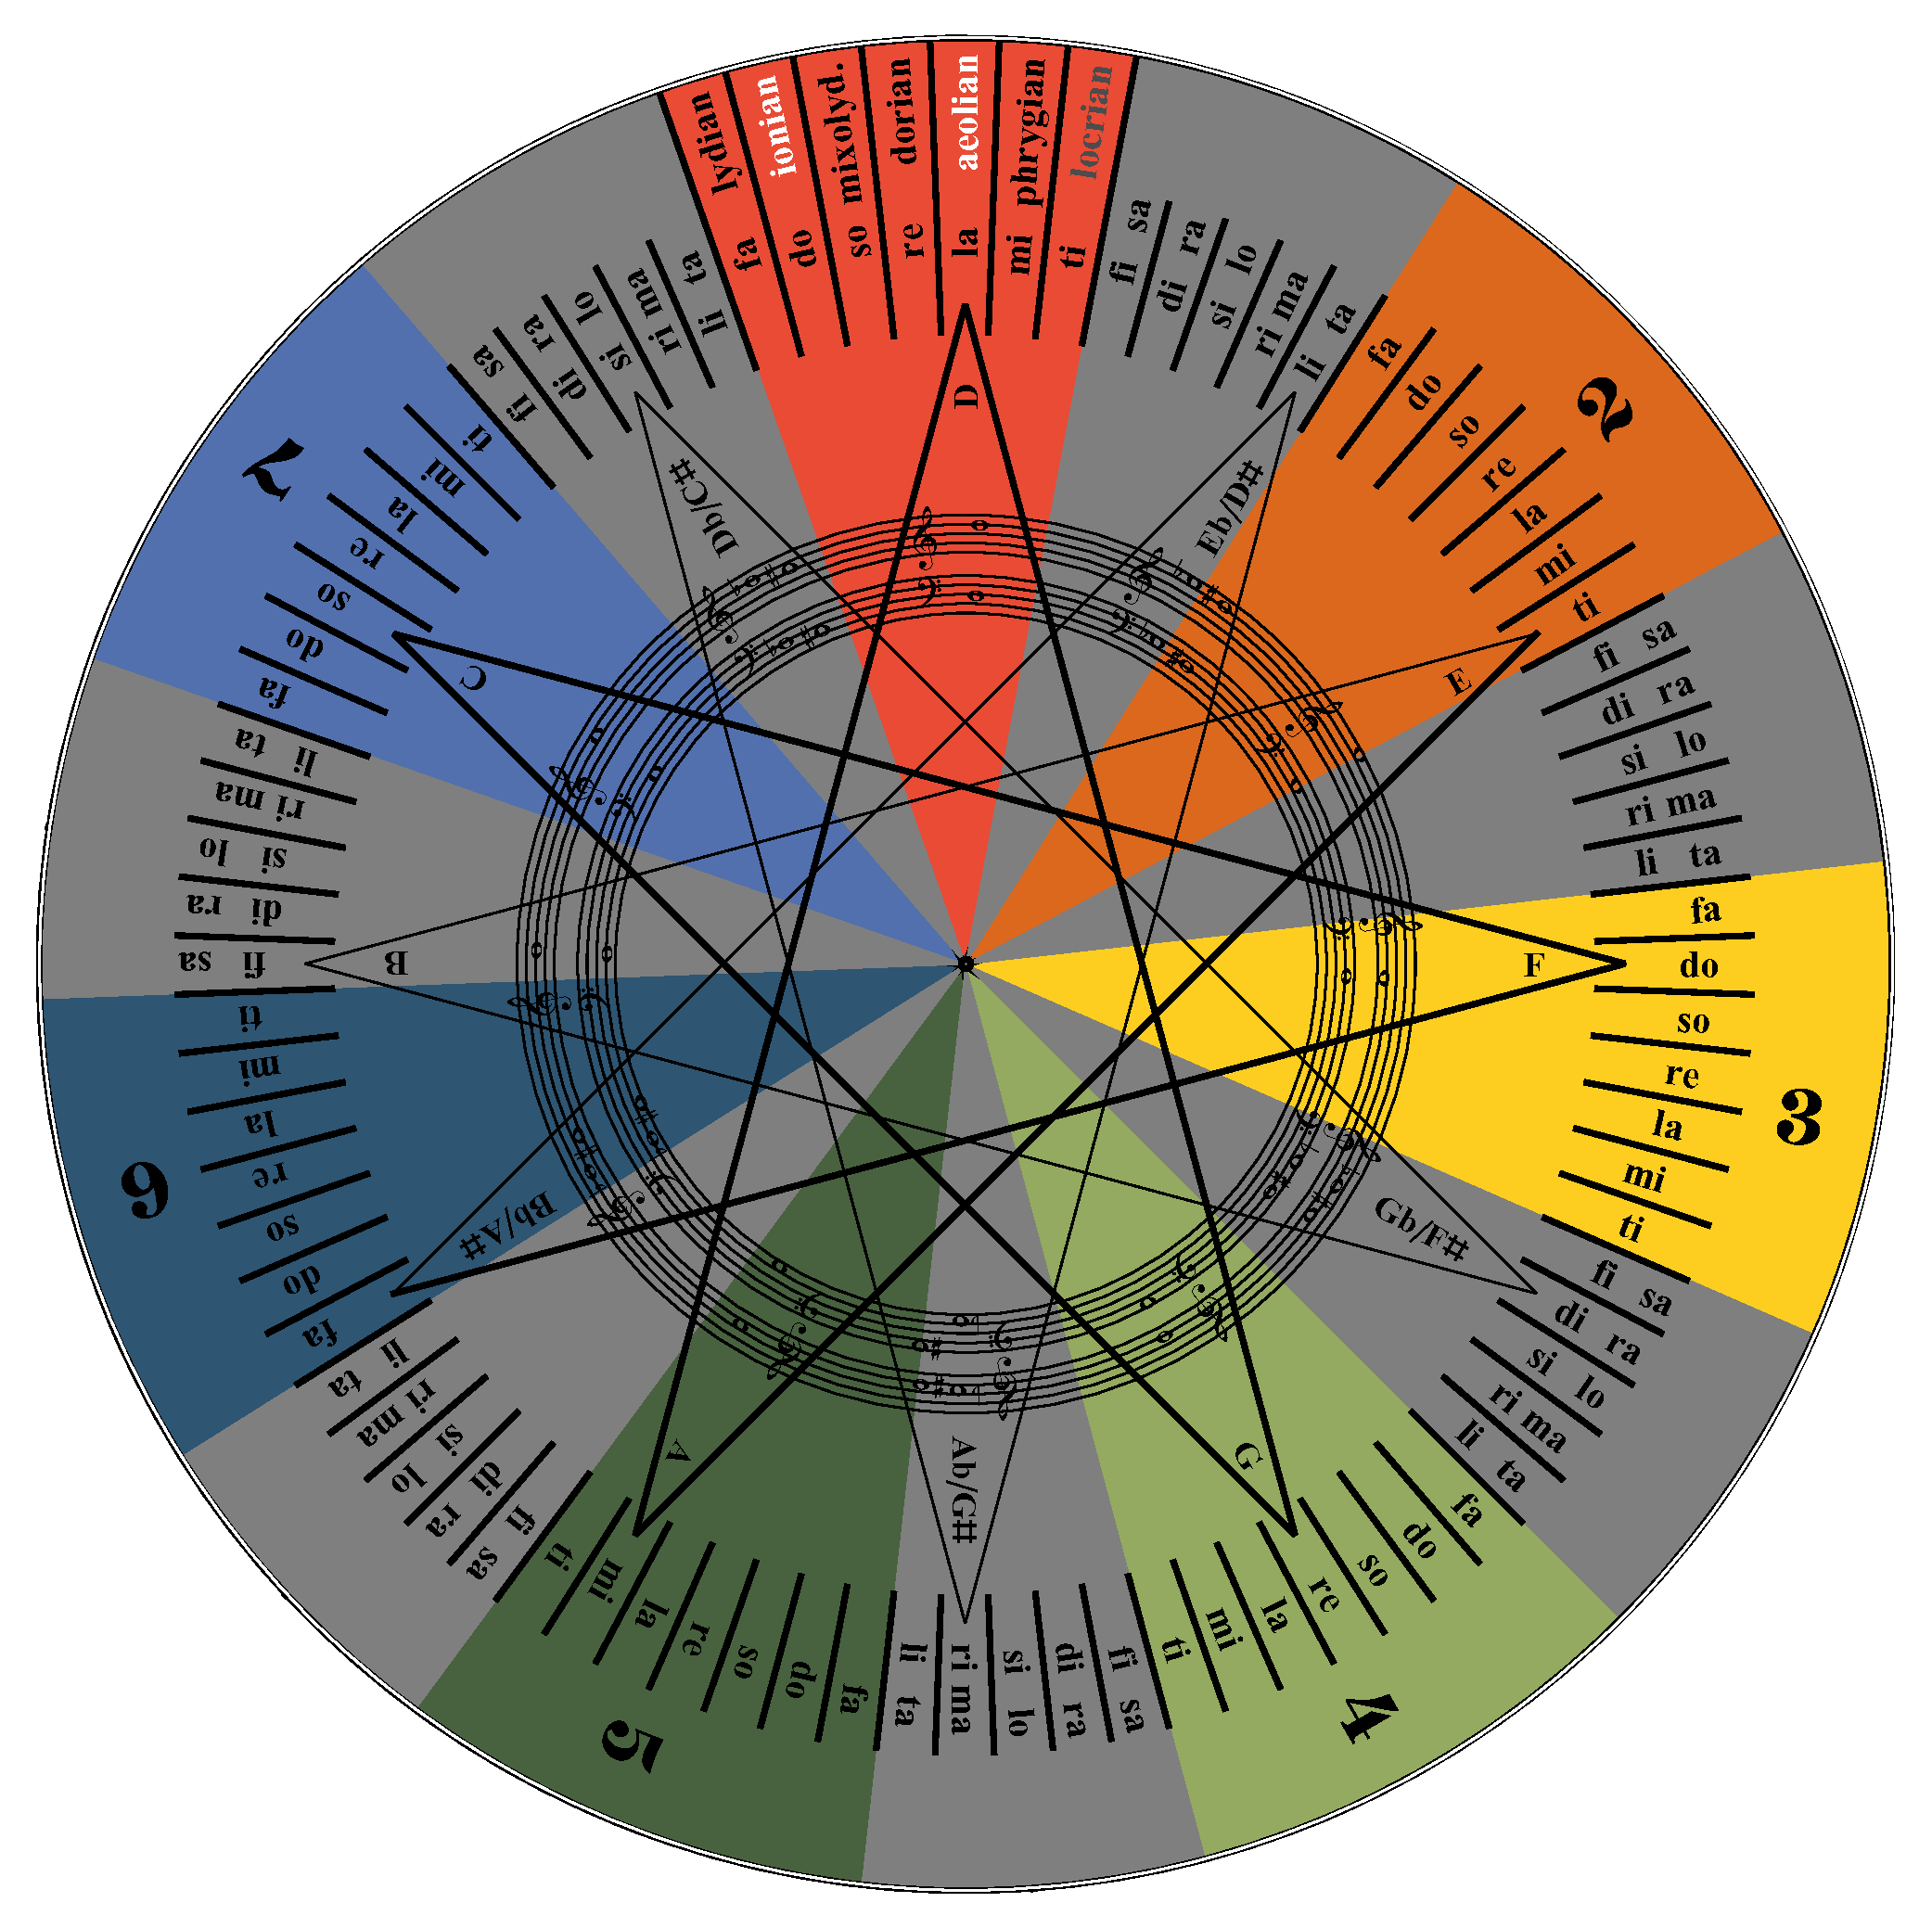
\includegraphics[width=0.95\textwidth]{NoteCompass_1}
\caption*{El Note Compass mostrant Re-Eoli. Les línies més gruixudes de l'estrella marquen la cadena de quintes de l'escala.}
\end{figure}


\begin{sectcredits}
\item[Autors del mòdul:] Thomas Noll (concepte) i Daniel Ramos per a IMAGINARY (Implementació).
\item[Text:] Thomas Noll i Daniel Ramos.
\end{sectcredits}

\section{Show me music}
Capbussa't en un munt de temes que mostren les complexes interrelacions de la melodia, l'harmonia i les matemàtiques. Cada animació s'assembla a certes peces o patrons des d'alguns punts de vista matemàtics. Alguns aspectes de simetria, tant en l'espai com en el temps, ajuden a entendre idees musicals.

\begin{figure}[!h]
\centering
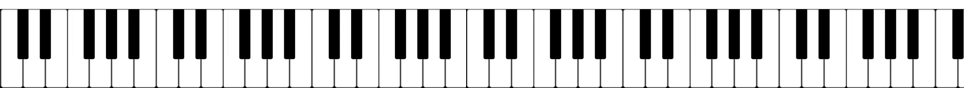
\includegraphics[width=\textwidth]{ShowMeMusic_1}
\end{figure}

\subsection{Spiral Tone Space}
Les tecles d'un piano formen un patró força regular. Entre cada grup de set lletres blanques el patró de tecles blanques i negres es repeteix. Si toques el piano i decideixes tocar vuit tecles blanques més a la dreta, la música sonarà gairebé igual... només que serà una octava més alta. Una bona manera d'expressar aquest fet de forma matemàtica és col·locar els tons en una espiral de manera que cada volta completa es correspon exactament amb una octava.

\begin{figure}[h]
\centering
\begin{subfigure}{0.45\textwidth}
\centering
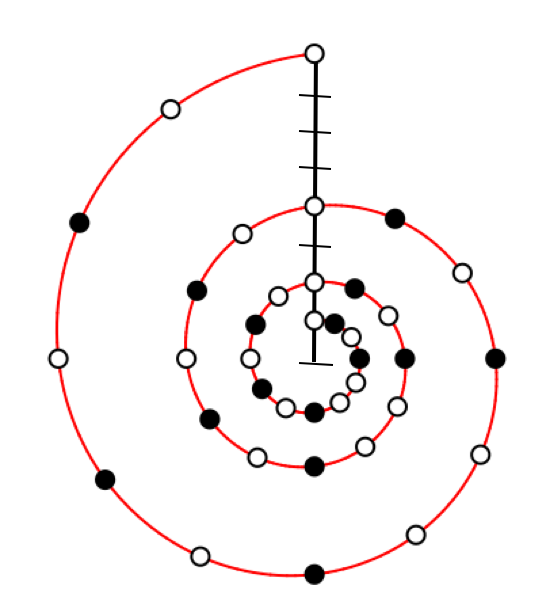
\includegraphics[height=4cm]{ShowMeMusic_2}
\end{subfigure}
\begin{subfigure}{0.45\textwidth}
\centering

\includegraphics[height=4cm]{ShowMeMusic_3}
\end{subfigure}
\end{figure}


\paragraph{La Música:} El concepte d'una octava és pràcticament omnipresent a la música. Fins i tot entre cultures diferents. Tocar una cançó una octava més amunt significa essencialment duplicar totes les freqüències. Això està estretament relacionat amb les sèries de sobretons. Un piano normalment té una mica més de 7 octaves. En canvi, el rang vocàlic humà és del voltant de 2 octaves.


\paragraph{Les Mates:} La figura de sobre il·lustra una seqüència de tres octaves en forma d'espiral logarítmica. Els tons greus estan situats més a prop del centre de l'espiral. Comença amb un Do i es mou en espiral en el sentit horari cap a notes més i més altes. Per poder-les seguir, s'ha utilitzat l'ordre de les tecles blanques i negres del piano. L'escala de l'espiral s'ha triat de manera que a cada volta completa es correspon a una octava i la distància de qualsevol punt fins al centre és proporcional a la seva freqüència. D'aquesta manera, al voltant del raig negre vertical, pots veure quatre Do diferents. Cadascun dels dotze raigs es correspon a cadascuna de les notes del nostre sistema de dotze tons. En funció del context, és comú i raonable no distingir entre notes igual de diferents octaves, això ens porta a l'anomenat espai tonal circular.

\paragraph{El Mòdul:} El mòdul visualitza els tons de cançons molt conegudes a l'espai tonal en espiral. Els paràmetres d'escala de l'espiral es trien de forma lleugerament diferent si cal veure més o menys octaves. Les notes predominants (a l'espai tonal circular) es detecten automàticament i s'assenyala adequadament la classe corresponent. Amb això pots seguir les notes dominants d'una cançó. Gaudeix escoltant i veient la música! Fins i tot cançons molt conegudes poden revelar patrons ocults i fer la composició més transparent.

\subsection{Space of Three-Note Chords}
A vegades apareixen estructures sorprenents si un estudia objectes des d'un punt de vista en què no només té en compte un objecte sinó diversos i les seves relacions. Per exemple, considerar totes les possibilitats per tocar un acord de tres notes dóna lloc a un objecte geomètric sorprenentment ric. Per això, ignorarem la informació de l'octava, de manera que tots els Do es tracten igual. La fotografia següent mostra aquest espai. Cada punt correspon a un possible acord. Resulta que aquest espai forma un prisma triangular que conté tots els 364 possibles acords. Cada punt correspon a tres notes . Els tres costats verticals corresponen a situacions on les tres notes són idèntiques. L'eix central de punts blancs correspon a acords de terceres encadenades. En aquest cas: Do - Mi - Sol$\sharp$


\begin{figure}[h]
\centering
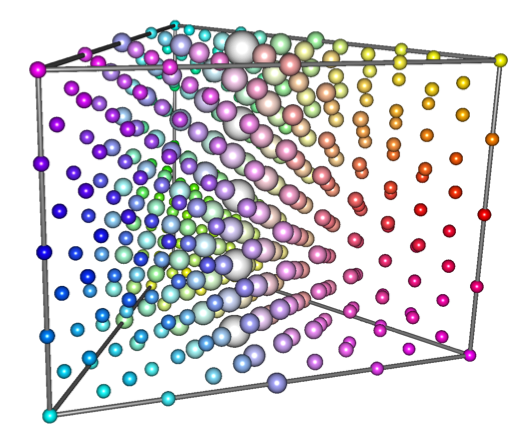
\includegraphics[width=0.6\textwidth]{ShowMeMusic_4}
\end{figure}

Els acords que es troben a prop d'altres en aquest espai es diferencien per un semitò. Fer petits canvis d'un acord a l'altre (amb moviments de semitò) significa voltar per l'estructura. Si fixem dues notes d'un acord i canviem l'altra en salts de semitò obtenim un camí lineal dins del prisma. Els costats quadrangulars actuen com parets o miralls on els camins reboten. Els costats superior i inferior estan també relacionats. Si intentes creuar el costat superior, aconsegueixes arribar a la part inferior, i viceversa.

\begin{wrapfigure}[18]{l}{0.35\textwidth}
\centering
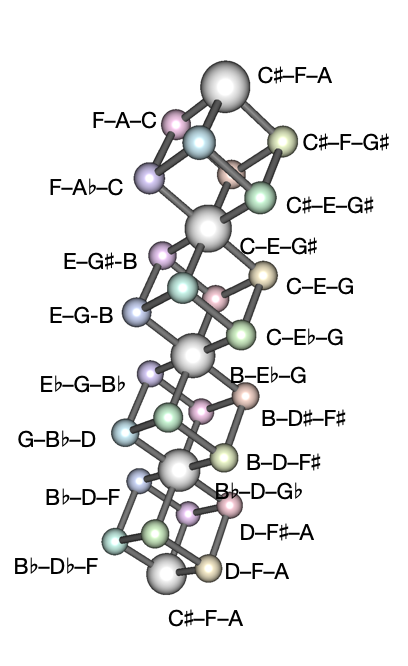
\includegraphics[width=0.34\textwidth]{ShowMeMusic_6}
\end{wrapfigure}
\paragraph{La Música:}  Aquesta estructura 3D codifica un munt de teoria musical clàssica. Per exemple, a una distància 1 de l'eix central pots trobar tots els acords majors i menors. A la fotografia s'etiqueten diversos acords. Les progressions clàssiques d'acords sovint es corresponen a passeigs per aquesta estructura.

\paragraph{Les Mates}: Aquesta imatge té moltes relacions profundes amb la teoria de la simetria. El fet que les cares quadrangulars actuïn com a miralls i que la superior i la inferior s'identifiquin fa que el prisma sigui fonamentalment una cel·la d'objectes tridimensionals en el qual infinits d'aquests prismes omplen tot l'espai. Just com un fons d'escriptori tridimensional simètric.  Considerar l'espai d'acords d'una manera tan genèrica és un  camp d'estudi relativament nou i que principalment dirigeix el professor Dimitri Tymoczko a Princeton.\\


\paragraph{El Mòdul:} El mòdul et permet navegar l'espai d'acords mencionat. La bola vermella indica la posició actual. Es toca un arpegi aleatori de l'acord seleccionat. Mou-te entre els acords, escolta'ls i crea les teves pròpies progressions musicals!

\begin{figure}[h]
\centering
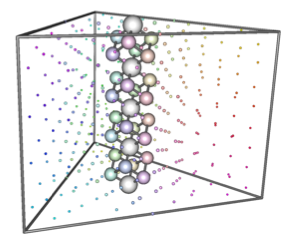
\includegraphics[width=0.5\textwidth]{ShowMeMusic_5}
\end{figure}


\subsection{Pachelbels Canon in D and Pachelballs}
El Cànon en Re de Pachelbel és, potser, una de les obres clàssiques més conegudes. Tot i que es va compondre l'any 1609 (segurament abans que l'obra de Back) sona sorprenentment fresc i modern. Segueix un esquema d'acords impressionant que fins i tot en l'actualitat forma part de la base de cançons molt conegudes de Pop, Folk, Country i Jazz com ara Skater Boy d'April Lavigne, No Woman No Cry de Bob Marley o Let it be dels Beatles.

\paragraph{Les Mates:} Un cànon és repetició i la repetició és simetria. En certa manera, un cànon és simetria en el temps. Es repeteix el mateix patró cada vegada que passa certa estona. De fet, el Cànon de Pachelbel és lleugerament diferent a la resta de cànons, ja que el patró musical de cada veu no es repeteix passada una estona.

\paragraph{La Música:} EL fet que les veus individuals no es repeteixin permeten a Pachelbel crear una progressió de densitat al cànon (a diferència d'altres). Pachelbel compon amb molts girs complicats tant rítmicament com melòdicament. A més a més, els patrons que fa la veu principal acaben convertint-se en l'acompanyament al cap d'uns moments.

\paragraph{El  Mòdul:} Dos dels nostres mòduls es basen en el Cànon de Pachelbel. Un d'ells visualitza la peça sencera i emfatitza el fet que les tres veus toquen exactament la mateixa partitura amb un desplaçament temporal, l'altre (Pachelballs) és un joc. Basant-te en els patrons d'acords de Pachelbel pots crear fragments molt agradables.

\begin{figure}[t]
\centering
\includegraphics[width=0.7\textwidth]{ShowMeMusic_7}
\end{figure}


\subsection{Mozart's Musical Dice Game}
Alguns anys després de la mort de Mozart es va publicar un dau musical. Aquest se li atribueix, ja que molt probablement era la seva invenció. En termes moderns, en podríem dir un generador de música aleatori. El joc permet la creació d'un minuet que sona bé i que el més possible és que no s'hagi tocat mai. Per això, Mozart presenta una partitura amb compassos numerats. Amb la partitura hi ha una taula per cada compàs amb possibles compassos que es poden utilitzar per omplir els espais buits. El compàs que s'utilitza en cada cas es determina tirant dos daus, sumant-ne el resultat i seleccionant la fila corresponent. Sorprenentment, l'estil de cada vals que es crea d'aquesta manera recorda molt a l'estil de Mozart.


\paragraph{La Música:} Com ho van fer? A primera vista, molta gent es va sorprendre per la música creada amb aquest procediment. Si hi donem una ullada més profunda, ja no resulta tan sorprenent. El contingut principal conceptualment es determina més aviat per la progressió harmònica que no per la melodia concreta de la cançó. Per una harmonia donada hi ha moltes maneres melòdiques d'expressar la mateixa idea. El que va fer Mozart és simplement oferir 11 possibilitats ``equivalents'' per cada compàs. És com substituir la frase ``L'ordinador està espatllat'' amb ``L'ordinador no funciona''. Per aquesta raó, els minuets creats amb aquest joc sonen més o menys igual.


\begin{wrapfigure}[22]{r}{0.4\textwidth}
\centering
\includegraphics[width=0.4\textwidth]{ShowMeMusic_8}
\end{wrapfigure}

\paragraph{Les Mates:} La primera pregunta i potser la més obvia és quantes possibles cançons es poden crear amb aquest joc? El vals té dues parts. Cadascuna té vuit compassos. Per cada compàs hi ha un total d'onze possibilitats. Amb una mica de combinatòria descobrim que hi ha l'astronòmic total de $11^{16} = 45 949 729 863 572 161$ possibilitats. Escoltar-les totes requeriria al voltant de 60 bilions d'anys. Creu-me, ja t'hauries avorrit.

També hi ha un subtil punt matemàtic en aquest joc. La distribució de compassos no serà una distribució igual. Com que cada compàs es tria amb la suma dels resultats de dos daus hi ha una tendència cap als nombres centrals. Hi ha un total de $6\times 6=36$ possibles resultats de les tirades dels dos daus. Només una d'aquestes, 1+1=2, creen el número 2, però n'hi ha sis que creen el número 7 = 1+6 = 2+5 = 3+4 = 4+3 = 5+2 = 6+1.

\paragraph{El Mòdul:} Si vols la teva peça individual de Mozart que, a més a més, no s'ha sentit mai, només has de prémer el botó i gaudir!

\subsection{Shepard Tone}

\begin{wrapfigure}[39]{l}{0.25\textwidth}
\centering
\includegraphics[height=0.9\textheight]{ShowMeMusic_9}
\end{wrapfigure}

La percepció és una cosa estranya. A vegades sentim o veiem coses que no hi són realment. Hi ha una il·lusió acústica que crea l'efecte d'un to que sempre puja o sempre baixa. El concepte és similar al de les escales d'Escher, que sembla que pugin amb cada pas, però realment només es mouen en cercles.

Aquesta il·lusió es crea de la següent manera: es defineix una finestra de freqüència, idealment amb límits suaus. Això es pot fer, per exemple, amb una campana de Gauss. En aquesta finestra tots els sobretons d'un cert espectre i que pertanyen al to es toquen. L'amplitud dels diferents tons parcials es determina segons la finestra. Ara l'espectre està desplaçat cap a la finestra. Mentre els sobretons greus s'esvaeixen gradualment, noves notes més agudes entren a la finestra. Mirant la mitjana, la freqüència es manté igual. Tot i això sona com un to descendent. Aquest edicte s'anomena To de Shepard

\paragraph{La Música:} És extremadament difícil tocar un To de Shepard convincent en un instrument clàssic i no electrònic. Requereix un control increïble sobre la intensitat de les notes tocades. Tanmateix, es va utilitzar per compositors moderns en diverses peces: la banda sonora de Hans Zimmer de la pel·lícula Dunkerque, el final de Echoes de Pink Floyd i fins i tot la banda sonora del joc Super Mario quan el protagonista corre per una escala sense fi.

\paragraph{Les Mates:}Crear un to de Shepard requereix precisió. Els tons han d'entrar i  sortir de l'espectre gairebé sense que ens n'adonem. Una bona manera de modelar-ho és utilitzant la campana de la distribució Gaussiana per controlar la intensitat dels sons que es toquen. Amb això, fins i tot un rang petit de freqüències fan un bon efecte. No obstant això, com més extens i més ric sigui l'espectre escollit més convincent és l'efecte. La fotografia mostra el sonograma d'un To de Shepard.

\paragraph{El Mòdul:}Amb el nostre mòdul pots controlar diversos paràmetres del To de Shepard controlant la forma i posició de la corba Gaussiana involucrada. Explora la llibertat que hi ha a l'hora de crear aquesta il·lusió acústica.

\begin{figure}[h]
\centering
\includegraphics[width=0.5\textwidth]{ShowMeMusic_10}
\end{figure}
\strut
\vspace{6em}

\begin{sectcredits}
\item[Autor del mòdul:] Jürgen Richter-Gebert (Technical University of Munich).

\item[Agraïments:] Patrick Wilson i Aaron Montag (sistema de so) Basat en CindyJS.org

\item[Text:] Jürgen Richter-Gebert (TU Munich).
\end{sectcredits}

\section{The Space of Pentatonic Scales}
Our usual tonal system consists of 12 halftone steps C-C\#-D-Eb... Each tone occurs exactly once in every octave. A nice way of visualizing this collection of tones is to arrange them in a circle and neglect the octave information. The image on the left shows the twelve notes with the usual distribution of black and white keys of a piano. The white circles form the material of the well-known C-major scale. But just playing the black notes also sounds interesting. They form a so called pentatonic scale: a collection of five notes within an octave. Forming melodies with them sounds a bit like modal music from the Far East. Rotating the pattern cyclically creates 12 similar sounding pentatonic scales.

\begin{figure}[h]
\centering
\begin{subfigure}{0.45\textwidth}
\centering
\includegraphics[width=0.9\textwidth]{PentatonicScales_1}
\end{subfigure}
\begin{subfigure}{0.45\textwidth}
\centering
\includegraphics[width=\textwidth]{PentatonicScales_2}
\end{subfigure}
\end{figure}

There are plenty of other ways to select exactly 5 notes out of the 12 notes in our tonal system. However, if we want to restrict ourselves to more or less equally distributed selections we can in addition require that no two ``neighboring'' notes are selected. Under these conditions there are, depending on rotation, exactly two more such arrangements of five tones. Each of them can occur in 12 different rotations (see picture).

\paragraph{The Music:} The pentatonic scales above have a kind of free floating sound that has no specific appeal of major or minor. Some of them sound very peaceful (the yellow one), some of them are full of tension. These scales were extensively used by the composers of the impressionistic epoch such as Debussy. They are used to create very colorful sounds invoking vivid pictures of other cultures. Debussy, for example became interested in pentatonic scales after hearing Gamelan Music from Java and Bali.

\paragraph{The Math:} The picture shows the space of all the above-mentioned halftone free pentatonic scales. Each of the three types occurs in 12 rotational positions. In the picture the scales are arranged in such a way that two of them are connected by an arc if they differ exactly by one halftone step. You see the ``space of pentatonic scales''.

\paragraph{The Exhibit:} In the Exhibit, a piece by a classical composer (Mozart, Bach, Debussy, Liszt, and others) can be chosen for playing. But the piece is not played according to notation. You choose a pentatonic scale and each note of the piece is replaced by the nearest tone on the scale. By tapping the rosettes, you can walk around and move from one pentatonic scale to another. Through this, you can create your own pieces of impressionistic music.

\begin{figure}
\centering
\includegraphics[width=0.6\textwidth]{PentatonicScales_3}
\end{figure}

\begin{sectcredits}
\item[Author of this exhibit:] Jürgen Richter-Gebert (Technical University of Munich)
\item[Acknowledgements:] Patrick Wilson and Aaron Montag (Sound Engine). Based on CindyJS.org
\item[Text:] Jürgen Richter-Gebert (TU Munich)
\item[Music:] Bach. Prelude and Fugue in C major BWV 846 / Mozart, Sonata No. 16 C major (Sonata facile), KV 545 / Liszt, Hungarian Rhapsody No 9 / Chopin, Prelude No 4  in e minor. Recorded by Bernd Krueger, Germany.
Gershwin. Rhapsody in Blue / Debussy, Arabesque 1 / Debussy, Images -- Reflets dans l'eau. Performed by Katsuhiro Oguri, Japan.
\end{sectcredits}

\section{The Sound of sequences}
La  On-line Encyclopedia of Integer Sequences (o OEIS) és una base de dades de seqüències de nombres trets de totes les branques d'investigació científica. Conté seqüències clàssiques com la llista de nombres primers o la seqüència amb els nombres de Fibonacci, o altres seqüències menys conegudes extretes de la resolució de problemes matemàtics, com ara el ``nombre de grafs planars amb n vèrtexs''. La base de dades la va començar l'any 1964 el matemàtic Neil J. A. Sloane com una eina per identificar i entendre seqüències. Avui inclou més de 300 000 seqüències.  

Les seqüències es poden analitzar matemàticament, visualitzant-les com a gràfiques de funció, o transformant-les en sons que es poden sentir, com en aquest cas. A més de revelar qualitats de la seqüència que no eren òbvies mirant els nombres, les peces de ``música'' són interessants a la seva manera. Esperem que n'escolteu algunes en aquest mòdul.  

Per transformar una seqüència a música, utilitzem un algorisme molt simple. Col·loquem la seqüència a les notes d'un piano. Aquest piano té 88 tecles i les numerem del zero fins al 87. Agafem els elements de la seqüència i hi sumem o hi restem múltiples de 88 fins que aconseguim un nombre dins del rang de 0 a 87. En termes tècnics, llegim la seqüència ``mòdul 88''.

\begin{figure}[h]
\centering
\includegraphics[width=0.7\textwidth]{SoundOfSequences}
\end{figure}

\vfill

Autors del mòdul: Neil J. A. Sloane (dades) i Eric Londaits per a IMAGINARY (Interfície d'usuari).
Text: Daniel Ramos (IMAGINARY).

Referències:
The On-line Encyclopedia of Integer Sequences. \url{www.oeis.org}.



\newpage
\pagecolor[RGB]{239,7,115}
\color{white}\resetnormalcolor
\vspace{-5cm}
\tableofcontents
\thispagestyle{empty}

\vspace{3em}
\urlstyle{same}
\noindent \textbf{ \large \url{ lalalab.imaginary.org}}

%\color{black}\resetnormalcolor

\vfill


\noindent\begin{tikzpicture}[remember picture, overlay]
\node[yshift=27mm, minimum width=73.5mm, minimum height=26mm, inner sep=0pt, fill=white, anchor=south west] at (current page.south west)  
	{\includegraphics[height=20mm]{logo-imaginary-magenta}};
	
\node[minimum width=73.5mm, minimum height=26mm, inner sep=0pt, fill=white, anchor=south west] at (current page.south west)  
	{\includegraphics[height=19mm]{logo-kts-magenta}};
	
\node[yshift=27mm, minimum width=73.5mm, minimum height=26mm, inner sep=0pt, fill=white, anchor=south east] at (current page.south east)  
	{\includegraphics[height=17mm]{logo-hlff-magenta}};
	
\node[minimum width=73.5mm, minimum height=26mm, inner sep=0pt, fill=white, anchor=south east] at (current page.south east)  
	{\includegraphics[height=14mm]{logo-tum-magenta}};

\end{tikzpicture}


\end{document}
